%!TeX program = xelatex

\documentclass[14pt, oneside]{extbook}

\usepackage{fontspec}
\setmainfont{Times New Roman}
\setmonofont{LMMonoLt10}[
  BoldFont=LMMonoLt10-Bold,
  ItalicFont=LMMonoLt10-Oblique,
  BoldItalicFont=LMMonoLt10-BoldOblique
]
\usepackage[english,russian]{babel}
\usepackage[a4paper, left=3cm, top=2cm, right=1.5cm, bottom=2cm]{geometry}

\usepackage{graphicx}
\usepackage{float}
\usepackage{amsmath}
\usepackage{amsfonts}
\usepackage{amssymb}
\usepackage{unicode-math}
\setmathfont{Latin Modern Math}
\usepackage[hidelinks]{hyperref}
\usepackage{caption}
\usepackage{ragged2e}
\usepackage{indentfirst}
\usepackage{setspace}
\usepackage{array}
\usepackage{longtable}
\usepackage{multirow}
\usepackage{microtype}
\newcolumntype{P}[1]{>{\raggedright\arraybackslash}p{#1}}

\onehalfspacing
\setlength{\parindent}{1.25cm}
\setlength{\emergencystretch}{3em}
\tolerance=2000
\everymath{\displaystyle}
\usepackage{tocloft}
\cftsetindents{chapter}{0pt}{2.5cm}
\cftsetindents{section}{1cm}{2.5em}
\renewcommand{\cftchappresnum}{Глава\ }
\renewcommand{\cftchapaftersnum}{.}
\renewcommand{\cftsecaftersnum}{.}

\renewcommand\cfttoctitlefont{\hfill\fontsize{18}{22}\selectfont\bfseries}
\renewcommand\cftaftertoctitle{\hfill\mbox{}}

\setlength{\cftbeforechapskip}{0pt}
\setlength{\cftbeforesecskip}{0pt}
\setlength{\cftbeforesubsecskip}{0pt}
\setlength{\cftbeforetoctitleskip}{0pt}
\setlength{\cftaftertoctitleskip}{0.6cm}
\setlength{\cftparskip}{0pt}
\setcounter{tocdepth}{2}

\renewcommand{\cftchapleader}{\cftdotfill{\cftchapdotsep}}
\renewcommand{\cftchapdotsep}{\cftdotsep}
\renewcommand{\cftchapfont}{\normalfont}
\renewcommand{\cftchappagefont}{\normalfont}

\makeatletter
\renewcommand{\@makeschapterhead}[1]{%
        \vspace*{0\p@}
        {\parindent \z@ \center
                \normalfont
                \fontsize{18}{22}\selectfont\bfseries #1\par\nobreak
                \addcontentsline{toc}{chapter}{#1}
                \vskip 10\p@
}}
\makeatother

\makeatletter
\renewcommand{\chapter}{%
        \if@openright\cleardoublepage\else\clearpage\fi
        \thispagestyle{plain}
        \global\@topnum\z@
        \@afterindentfalse
\secdef\@chapter\@schapter}

\renewcommand{\@makechapterhead}[1]{%
        \vspace*{0\p@}
        {\parindent \z@ \raggedright
                \normalfont
                \fontsize{18}{22}\selectfont\bfseries Глава \thechapter. #1\par\nobreak
                \vskip 20\p@
}}
\makeatother

\makeatletter
\newcommand{\custompagestyle}{%
        \begingroup
        \renewcommand{\ps@plain}{%
                \renewcommand{\@oddfoot}{\hfill\thepage}
                \renewcommand{\@evenfoot}{\hfill\thepage}
                \renewcommand{\@oddhead}{}
                \renewcommand{\@evenhead}{}
        }%
        \pagestyle{plain}
}
\makeatother

\makeatletter
\renewcommand\section{\@startsection {section}{1}{\z@}%
                                   {-3.5ex \@plus -1ex \@minus -.2ex}%
                                   {2.3ex \@plus.2ex}%
                                   {\normalfont\fontsize{16}{20}\selectfont\bfseries}}
\renewcommand\@seccntformat[1]{\csname the#1\endcsname.\ }
\makeatother

\captionsetup{font={small}}

\newenvironment{customquote}
{\list{}{\leftmargin=0pt
                \rightmargin=0pt
                \topsep=0pt
                \partopsep=0pt
                \parsep=2pt
                \itemsep=0pt
        }%
        \normalfont\relax
\item\relax}
{\endlist}

\begin{document}
\thispagestyle{empty}
\begin{center}
        \textbf{САНКТ-ПЕТЕРБУРГСКИЙ ГОСУДАРСТВЕННЫЙ УНИВЕРСИТЕТ}

        \vspace{1em}
        \textit{Факультет прикладной математики --- процессов управления}

        \vspace{1em}
        \textit{Кафедра моделирования электромеханических и компьютерных систем}

        \vspace{4em}
        \textbf{\textit{\large Шаго Павел Евгеньевич}}

        \vspace{2em}
        \textbf{\Large Выпускная квалификационная работа}

        \vspace{1em}
        \textbf{\Large «Математическое моделирование и реализация планировщика
        процессов для гетерогенных процессорных архитектур»}

        \vspace{2em}
        Уровень образования: бакалавриат \\
        Направление: 01.03.02 Прикладная математика и информатика \\
        Основная образовательная программа СВ.5005.2022:
        «Прикладная математика, фундаментальная информатика и программирование»

        \vspace{2em}
        \begin{flushright}
                Научный руководитель \\
                кандидат физ.-мат. наук, доцент \\
                Корхов Владимир Владиславович
        \end{flushright}

        \begin{flushright}
                Рецензент \\
                Эксперт по архитектуре и сетевому стеку \\
                ООО НИЦ АЭРОДИСК \\
                Анохин Юрий Владимирович
        \end{flushright}

        \vfill
        Санкт-Петербург\\ \the\year
\end{center}

\newpage
\custompagestyle
\setcounter{page}{2}
\renewcommand{\contentsname}{Содержание}
\tableofcontents

\newpage
\chapter*{Список сокращений}

\begin{longtable}{@{}p{2.8cm}>{\raggedright\arraybackslash}p{12.6cm}@{}}
eBPF (BPF) & расширенный фильтр пакетов Беркли (extended Berkeley Packet Filter) \\
CPU & центральный процессор (Central Processing Unit) \\
DSQ & очередь диспетчеризации в sched\_ext (dispatch queue) \\
EEVDF & планировщик ближайшего допустимого виртуального дедлайна (Earliest Eligible Virtual Deadline First) \\
EWMA & экспоненциально взвешенное скользящее среднее (exponentially weighted moving average) \\
FIFO & первым пришёл, первым обслужен (First In First Out) \\
LAVD & планировщик с учётом критичности задержки (Latency-criticality Aware Virtual Deadline) \\
MDP & марковский процесс принятия решений (Markov Decision Process) \\
P/E & производительные / энергоэффективные ядра (Performance / Efficient) \\
QPS & запросов в секунду (queries per second) \\
RAPL & интерфейс ограничения средней мощности (Running Average Power Limit) \\
RISC & архитектура с сокращённым набором команд (Reduced Instruction Set Computer) \\
RPS & запросов в секунду (requests per second) \\
SCX & расширяемый класс планирования (Scheduler Class eXtensible, sched\_ext) \\
SMT & одновременная многопоточность (Simultaneous Multithreading, Hyper-Threading) \\
SoC & система на кристалле (System on a Chip) \\
TPS & транзакций в секунду (transactions per second) \\
VCG & механизм Викри--Кларка--Гровса (Vickrey--Clarke--Groves) \\
\end{longtable}

\newpage
\chapter*{Введение}

        Планировщик операционной системы (ОС) распределяет
        процессорное время между задачами. От качества его решений
        зависят пропускная способность системы под нагрузкой,
        время отклика интерактивных приложений и энергопотребление
        оборудования.

        Современные процессоры всё чаще имеют гетерогенную
        архитектуру, при которой на одном кристалле сочетаются
        производительные и энергоэффективные ядра. Такая
        организация уже применяется в мобильных процессорах ARM
        big.LITTLE, в настольных и серверных процессорах Intel
        начиная с поколения Alder Lake, появляется и в экосистеме
        RISC-V. Выбор ядра при размещении задачи влияет на время
        её выполнения и энергопотребление, поэтому планировщик
        должен учитывать различие ядер.

        Интерактивные, пакетные и фоновые нагрузки предъявляют
        к планировщику различные требования, и оптимальная для
        одного сценария политика редко оказывается удачной для
        другого. Возникает потребность подбирать политику под
        конкретный сценарий, однако штатный планировщик ядра
        Linux един для всех пользователей, а его самостоятельная
        модификация трудоёмка в сопровождении и плохо переносима
        между версиями ядра.

        В ответ на эту потребность в ядро Linux был принят
        фреймворк sched\_ext, позволяющий реализовывать политику
        планирования как программу, загружаемую в ядро во время
        работы системы без его пересборки. Это ускоряет
        разработку и снижает порог входа для прототипирования
        новых алгоритмов.

        В настоящей работе предлагается аукционная модель
        планировщика A1349\footnote{\textbf{A}
        (Auction)~--- аукционный механизм. \textbf{1}~---
        единая функция Беллмана. \textbf{3}~--- три
        кластерные DSQ. \textbf{4}~---
        четырёхуровневый приоритет извлечения. \textbf{9}~---
        Допущение~\ref{assum:atomic} об атомарном
        контракте.},
        учитывающая различие ядер по
        вычислительной мощности, как альтернатива базовому
        планировщику Linux. Средствами sched\_ext реализованы
        обе модели, A1349 и базовая для Linux модель EEVDF.
        Реализация EEVDF позволяет дополнительно оценить
        накладные расходы фреймворка. Обе реализации сравниваются
        со штатным планировщиком на наборе тестов при различных
        типах нагрузок.


\chapter*{Постановка задачи}

        Объектом исследования являются алгоритмы планирования
        задач (процессов)
        в операционных системах на вычислительных устройствах с гетерогенной
        процессорной архитектурой (Intel Hybrid, ARM big.LITTLE
        и другие).

        Предметом исследования являются методы планирования
        задач, учитывающие различие вычислительной мощности ядер
        процессора.

        Целью работы является разработка и экспериментальная оценка
        планировщика, обеспечивающего более высокую эффективность вычислений
        на гетерогенном оборудовании по сравнению с базовым
        алгоритмом EEVDF ядра Linux.

        Для достижения цели работы необходимо:
        \begin{enumerate}
                \item Проанализировать и определить наиболее перспективный
                        подход к реализации планировщика.
                \item Построить математическую модель, учитывающую
                        различную вычислительную мощность ядер процессора.
                \item Реализовать разработанный алгоритм и
                        собрать воспроизводимый набор бенчмарков.
                \item Провести эксперимент на гетерогенном оборудовании
                        и оценить результаты в сравнении с базовым
                        планировщиком Linux EEVDF.
        \end{enumerate}


\chapter{Подходы к реализации планировщиков в ОС}
\section{Задача планирования}

        Операционные системы реализуют многозадачность через
        контекстное переключение, выделяя задачам кванты
        процессорного времени. Задача планирования состоит в
        построении расписания, минимизирующего простои
        оборудования и максимизирующего целевые показатели
        эффективности. Обычно её решает встроенный в ядро ОС
        компонент, называемый планировщиком, который распределяет
        задачи по ядрам процессора.

        С развитием операционных систем и оборудования планировщики также
        эволюционировали.
        Так, в операционной системе UNIX планировщик выбирал задачу
        по приоритету,
        а среди равных задач использовался алгоритм похожий на
        round-robin~\cite{lions}.
        Позднее в ядре Linux версии 2.4 был реализован планировщик
        O(n), который при планировании
        следующей задачи просматривал очередь готовых к исполнению задач
        и вычислял для них эвристику \textit{goodness}~\cite{kravetz_elss}.
        В Linux 2.6 его сменил планировщик O(1), в котором разделили
        очередь приоритетов на два массива, \textit{active} и
        \textit{expired}, что позволило выбирать
        следующую задачу за постоянное время~\cite{love}.

        Затем в версии Linux 2.6.23 произошёл переход к планировщику
        Completely Fair Scheduler (CFS), основанному на модели виртуального
        времени. Готовые к выполнению задачи хранились в красно-чёрном дереве,
        упорядоченном по виртуальному времени, а планировщик выбирал задачу,
        получившую меньше всего процессорного времени относительно своей
        справедливой доли~\cite{wong}.
        В Linux 6.6 эта идея получила развитие в планировщике Earliest
        Eligible Virtual Deadline First (EEVDF), где вводятся
        отставание и виртуальный дедлайн. Допустимыми считаются задачи,
        у которых отставание lag $ \geq 0 $, среди них выбирается задача с
        ближайшим виртуальным дедлайном~\cite{stoica}.

        Таким образом, за последние полвека планировщик операционной
        системы прошёл путь от детерминированных приоритетных схем,
        близких по логике к round-robin, до алгоритмов динамического
        распределения процессорного времени, основанных на серьёзных
        математических моделях.


\section{Гетерогенные процессорные архитектуры}

        Если классические многопроцессорные системы строились на
        симметричном принципе (SMP), где все ядра обладают
        одинаковой производительностью и энергопотреблением,
        то современные процессоры всё чаще объединяют на одном
        кристалле ядра разных классов. Архитектура ARM big.LITTLE
        впервые сделала такой подход массовым в мобильном
        сегменте, объединив производительные ядра (\textit{big})
        с энергоэффективными (\textit{LITTLE})~\cite{biglittle}.
        В настольных и серверных процессорах Intel начиная с
        поколения Alder Lake внедрена гибридная архитектура с
        Performance и Efficient ядрами (P/E)~\cite{intelhybrid}.
        Принцип не привязан к конкретной системе команд.
        Аналогичные конфигурации появляются и в экосистеме
        RISC-V, например, гетерогенный SoC Marsellus~\cite{marsellus}.

        Ядра одного процессора в таких системах отличаются по
        тактовой частоте, ширине внеочередного исполнения, размеру
        кэшей и энергопотреблению. Одна и та же задача, выполненная
        на P-ядре, завершается быстрее, но с большими
        энергозатратами, тогда как E-ядро обеспечивает лучшее соотношение
        производительность/ватт при более низкой пропускной
        способности. Размещение чувствительной к задержкам задачи
        на E-ядре увеличивает время её обслуживания, а выполнение
        фоновой нагрузки на P-ядре приводит к избыточному
        энергопотреблению.

        В ядре Linux различия между ядрами обрабатываются
        подсистемой Capacity Aware Scheduling (CAS), учитывающей
        относительную мощность каждого ядра при балансировке.
        Поверх неё работает Energy Aware Scheduling (EAS), которая
        по модели энергопотребления и оценкам загрузки выбирает
        для задачи ядро с меньшим потреблением без потери
        пропускной способности. EAS включается лишь при наличии
        энергомодели, регулятора частоты schedutil и отсутствии
        SMT (Hyper-Threading), поэтому применяется прежде всего на
        мобильных SoC ARM big.LITTLE~\cite{eas}. На стороне x86
        для информирования планировщика о приоритете ядер
        применяется механизм Intel Thread Director, транслирующий
        аппаратные подсказки о характере нагрузки в теги класса
        задачи~\cite{intelhybrid}. Однако CAS и Thread Director закрывают лишь
        балансировку по вычислительной мощности и классификацию по
        профилю инструкций, тогда как раздельные очереди готовых задач
        для P/E-кластеров,
        приоритизация чувствительных к задержкам нагрузок и прикладные
        правила выбора кластера остаются за пределами штатной
        подсистемы. Реализация подобных политик требует существенных
        изменений ядра, что мотивирует переход к расширяемым
        механизмам, рассматриваемым в следующем разделе.


\section{Расширяемый планировщик Linux}\label{sec:schedext}

        \textbf{sched\_ext} (scheduler extensions)~\cite{schedext} --
        инфраструктура (фреймворк) ядра Linux, позволяющая
        реализовывать политику планирования как eBPF-программу,
        подключаемую к интерфейсу расширяемых планировщиков во
        время работы системы без пересборки ядра. sched\_ext был
        включён в основную ветку Linux в версии 6.12 и
        предоставляет отдельный класс планирования
        \texttt{ext\_sched\_class}, расположенный между классами
        \texttt{fair\_sched\_class} и \texttt{idle\_sched\_class}.
        При загруженном eBPF-планировщике обычные задачи
        переводятся из класса справедливого планирования
        \texttt{fair\_sched\_class} (далее fair-класс) под
        управление sched\_ext.

        \begin{figure}[h]
                \centering
                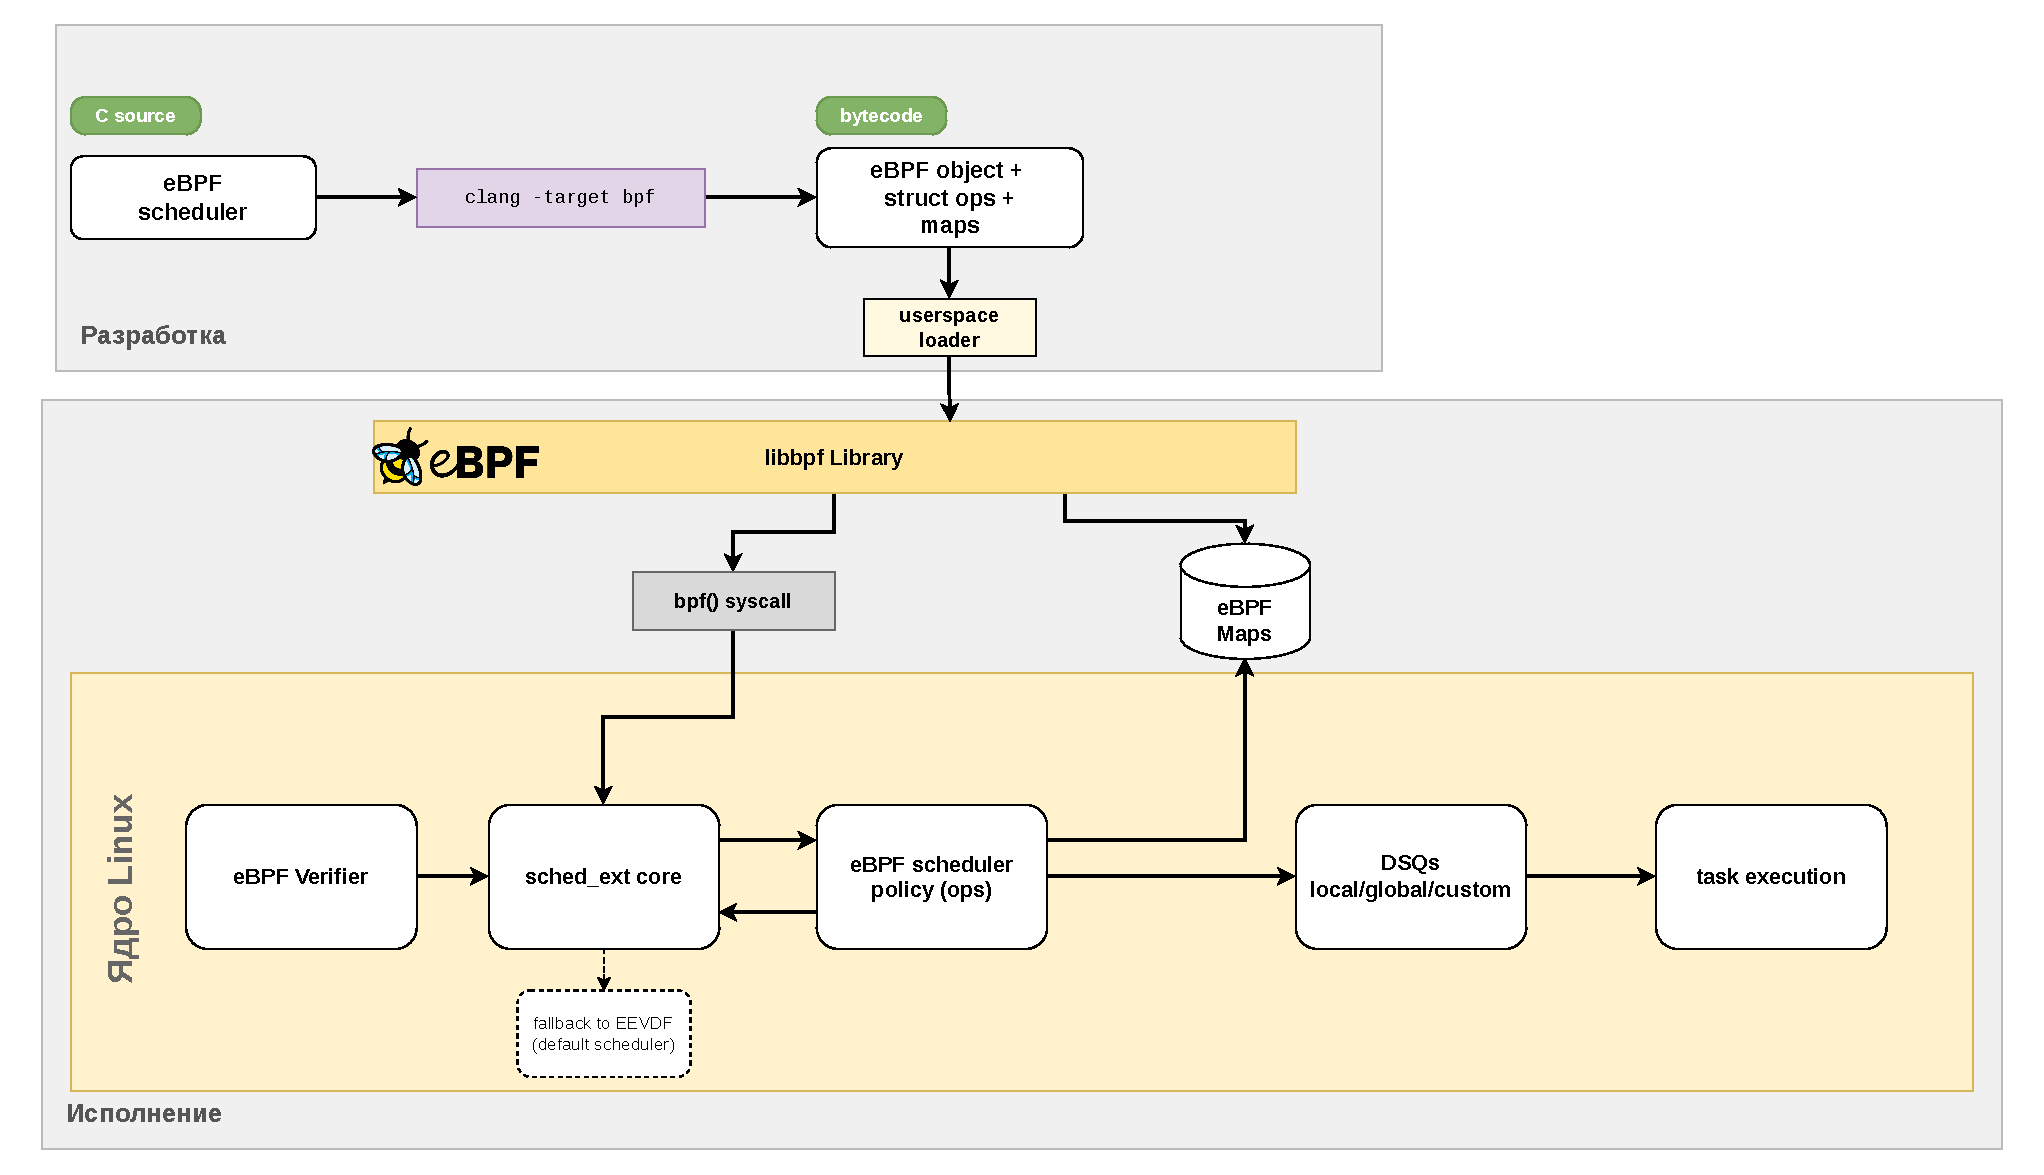
\includegraphics[width=\textwidth, height=0.42\textheight]{res/sched_ext.pdf}
                \caption{Архитектура sched\_ext в ядре Linux}
                \label{fig:sched_ext}
        \end{figure}

        Подход с вынесением политики планирования из ядра
        встречался и до sched\_ext. В системе ghOSt~\cite{ghost}
        политика реализована как пользовательский процесс-агент.
        Через разделяемую память он наблюдает состояние задач и
        назначает следующую задачу на процессорное ядро, а ядро ОС
        лишь выполняет переключение контекста. Это позволяет
        описывать политику на обычном языке программирования и
        опираться на пользовательские средства отладки.

        Важно отметить, что sched\_ext замещает только fair-класс.
        Задачи реального времени (\texttt{SCHED\_FIFO}, \texttt{SCHED\_RR})
        и задачи с дедлайнами (\texttt{SCHED\_DEADLINE}) остаются
        под управлением штатных классов \texttt{rt\_sched\_class} и
        \texttt{dl\_sched\_class}. Это ограничивает область
        применимости пользовательских политик, но сохраняет
        гарантии для критичных по времени задач.

        Безопасность исполнения произвольной политики
        обеспечивается несколькими механизмами времени выполнения.
        Таймер \texttt{watchdog} отслеживает случаи, когда задача
        не получает процессорного времени дольше установленного
        порога (по умолчанию 30 секунд). При штатной выгрузке,
        критической ошибке внутри планировщика или срабатывании
        \texttt{watchdog} ядро автоматически возвращает все задачи
        под управление EEVDF, что обеспечивает безопасность
        экспериментов на работающей системе. Дополнительно
        реализована возможность экстренного отключения
        пользовательской политики комбинацией клавиш
        \texttt{SysRq-S}.

        С точки зрения программной модели, политика планирования
        в sched\_ext описывается набором обратных вызовов,
        объединённых в структуру \texttt{struct sched\_ext\_ops}.
        К основным обработчикам относятся \texttt{select\_cpu},
        вызываемый при пробуждении задачи и отвечающий за выбор
        ядра исполнения, \texttt{enqueue}, помещающий задачу в
        очередь готовых к выполнению, \texttt{dispatch},
        выбирающий следующую задачу для конкретного ядра, а также
        \texttt{running} и \texttt{stopping}, дающие
        дополнительные контрольные точки для обновления метрик
        (при начале и завершении исполнения задачи).
        Дополнительные обработчики \texttt{init\_task},
        \texttt{exit\_task}, \texttt{cpu\_online} и
        \texttt{cpu\_offline} позволяют поддерживать собственное
        состояние, связанное с задачами и ядрами, на протяжении
        всего их жизненного цикла. Отдельная группа обработчиков
        \texttt{cgroup\_init}, \texttt{cgroup\_exit},
        \texttt{cgroup\_move} и \texttt{cgroup\_set\_weight}
        обеспечивает интеграцию с иерархией контрольных групп.
        Они вызываются при создании и удалении cgroup, перемещении
        задач между группами, а также при изменении веса группы,
        что позволяет реализовывать иерархические политики
        планирования.

        Поведение фреймворка настраивается через флаги поля
        \texttt{ops->flags}. Флаг \texttt{SCX\_OPS\_SWITCH\_PARTIAL}
        переводит под управление sched\_ext только задачи с явной
        политикой \texttt{SCHED\_EXT}, оставляя
        \texttt{SCHED\_NORMAL}, \texttt{SCHED\_BATCH} и \texttt{SCHED\_IDLE}
        в fair-классе. Флаг \texttt{SCX\_OPS\_ENQ\_LAST} определяет,
        попадает ли последняя выполнявшаяся задача обратно в очередь
        после исчерпания кванта. Флаг
        \texttt{SCX\_OPS\_KEEP\allowbreak\_BUILTIN\_IDLE}
        указывает ядру продолжать обновлять битовую маску простаивающих
        CPU при загруженной пользовательской политике. Без этого флага
        eBPF-программе пришлось бы вести учёт самостоятельно, тогда как
        с ним поиск свободного ядра доступен через штатные
        kfunc-вызовы (стабильные функции ядра, доступные из eBPF).

        Передача задач между обработчиками происходит через DSQ.
        Помимо встроенных глобальной \texttt{SCX\_DSQ\_GLOBAL}
        и локальных по числу ядер \texttt{SCX\_DSQ\_LOCAL},
        eBPF-программа может создавать произвольное количество собственных
        очередей с заданным идентификатором при помощи
        \texttt{scx\_bpf\_create\_dsq}.
        Каждая DSQ обслуживается по принципу FIFO либо по виртуальному времени,
        задаваемому при вставке через
        \texttt{scx\_bpf\_dsq\allowbreak\_insert\_vtime}.
        В режиме виртуального времени очередь реализована как
        красно-чёрное дерево, упорядоченное по полю \texttt{vtime},
        что обеспечивает извлечение задачи с наименьшим виртуальным
        временем за $O(\log n)$.
        Возможность создавать произвольные DSQ позволяет завести
        отдельную очередь на каждый кластер ядер и обслуживать её
        по собственному виртуальному времени. Тогда задача,
        помещённая в очередь нужного кластера на этапе \texttt{enqueue},
        попадёт на исполнение только к ядрам этого кластера, а
        упорядочивание по \texttt{vtime} сохраняется внутри кластера
        независимо от остальных. Такое разделение существенно
        в контексте гетерогенных архитектур, где P/E-ядра
        отличаются по производительности и требуют раздельного учёта.

        \begin{sloppypar}
                Для взаимодействия с ядром eBPF-программа использует
                kfunc-вызовы. Так, \texttt{scx\_bpf\_dsq\_insert}
                помещает задачу в выбранную очередь, а
                \texttt{scx\_bpf\_dsq\_move\_to\_local} извлекает
                задачу для исполнения на текущем ядре.
                Состояние задач и ядер хранится в \texttt{BPF\_MAP}-структурах,
                а доступ к полям \texttt{task\_struct} и \texttt{rq}
                осуществляется
                через механизм CO-RE (Compile Once -- Run
                Everywhere), что обеспечивает
                переносимость скомпилированной программы между версиями ядра.
        \end{sloppypar}

        Для типичных нужд балансировки фреймворк предоставляет
        встроенный учёт простаивающих ядер. Функции
        \texttt{scx\_bpf\_pick\_idle\_cpu} и
        \texttt{scx\_bpf\_test\_and\allowbreak\_clear\_cpu\_idle}
        позволяют без собственной реализации находить свободные
        CPU по битовой маске.
        Если обработчик \texttt{select\_cpu} помещает задачу
        непосредственно в локальную очередь \texttt{SCX\_DSQ\_LOCAL}
        целевого ядра, последующий вызов \texttt{enqueue} для этой
        задачи пропускается, что образует быстрый путь пробуждения
        и сокращает накладные расходы на часто пробуждающихся задачах.

        Собственное состояние, привязанное к конкретной задаче,
        удобно хранить в структуре типа \texttt{BPF\_MAP\_TYPE\_TASK\_STORAGE},
        которая обеспечивает константное время доступа без хеш-поиска
        и автоматически освобождается при завершении задачи.
        Длительность кванта процессорного времени задаётся
        присваиванием поля \texttt{p->scx.slice} в обработчиках
        \texttt{enqueue} или \texttt{dispatch}. По умолчанию
        используется \texttt{SCX\_SLICE\_DFL} (20\,мс). Вытеснение уже
        исполняющейся задачи на удалённом ядре инициируется
        вызовом \texttt{scx\_bpf\_kick\_cpu} с флагом
        \texttt{SCX\_KICK\_PREEMPT}.

        На этапе загрузки программы среда eBPF накладывает на
        политику планирования ряд архитектурных ограничений,
        проверяемых верификатором. В программе запрещены блокирующие
        вызовы и динамическая аллокация памяти, любой цикл должен
        иметь верифицируемую верхнюю границу, а доступ к структурам
        ядра разрешён только через утверждённый набор kfunc и полей.
        Эти требования заметно сказываются на выборе структур данных
        и способов агрегирования метрик при разработке планировщика.


\section{Актуальные исследования планировщиков}

        С появлением фреймворка sched\_ext~\cite{schedext}
        исследовательская активность
        в области планировщиков задач заметно возросла. Большинство
        современных работ используют sched\_ext как экспериментальную платформу
        для быстрой проверки новых алгоритмов без модификации ядра.
        Диапазон применения охватывает оптимизации существующих алгоритмов,
        подходы машинного обучения и нестандартные постановки задач.

        Tang~et~al.~\cite{srand} предложили sched\_ext-планировщик
        SRAND, в котором расчёт отставаний и виртуальных дедлайнов
        EEVDF заменён упрощённой схемой виртуального времени и
        многоуровневой очередью. По завершении кванта виртуальное
        время задачи увеличивается на
        $(slice - p.slice) \cdot 100 / p.weight$, где
        $slice = 20\,$мс — длительность кванта, $p.slice$ — его
        неиспользованный остаток, $p.weight$ — вес задачи. У задач
        с большим весом виртуальное время растёт медленнее, что
        соответствует более высокому приоритету. Новые и
        пробуждающиеся задачи инициализируются текущим глобальным
        виртуальным временем системы, которое подтягивается до
        максимума активных задач. Если у пробудившейся задачи
        виртуальное время меньше $V(t) - slice$, оно поднимается
        до этого порога, что не даёт долго неактивной задаче
        монополизировать ядро.

        Полученное виртуальное время определяет распределение
        по пяти BPF-очередям с порогами 20, 50, 200 и 500\,мс
        (\texttt{queue0}--\texttt{queue4}). Задачи из очередей с
        меньшим индексом первыми переходят в единую глобальную
        FIFO-очередь, откуда ядра напрямую извлекают следующую.
        Это заменяет обход красно-чёрного дерева EEVDF одной
        операцией взятия с головы. Дополнительно поддерживаются
        локальные очереди свободных ядер с привязкой задач к
        ядрам, на которых они уже работали. Потоки ядра получают
        неограниченный квант и направляются непосредственно в
        локальную очередь. Политика реализована через обработчики
        \texttt{select\_cpu}, \texttt{enqueue} и \texttt{dispatch}.
        Время ожидания в очереди ограничено 5000\,мс. По данным
        авторов, на Lmbench время переключения контекста
        сокращается на 11,83\%, а на hackbench общая
        производительность растёт на 7,02\% при сопоставимой с
        EEVDF равномерности распределения нагрузки (дисперсия загрузки
        ядер $s^2 = 0{,}005$ против $0{,}006$ у EEVDF).

        Xu~et~al.~\cite{lace} применили sched\_ext к задаче
        управляемого тестирования параллелизма (\emph{controlled
        concurrency testing}, CCT) ядра Linux. Планировщик LACE
        переключает конфликтующие потоки в контролируемом порядке,
        автоматически вставляя точки переключения в операциях с
        разделяемой памятью и примитивах синхронизации, что
        позволяет систематически воспроизводить состояния гонки
        без вмешательства гипервизора. По сравнению с фаззером
        SegFuzz LACE увеличивает покрытие ветвлений на 38\%,
        снижает накладные расходы на 57\% и ускоряет
        воспроизведение ошибок в 11,4 раза, обнаружив восемь ранее
        неизвестных ошибок параллелизма при объёме патчей ядра
        менее 25 строк. Работа
        показывает, что sched\_ext пригоден не только для оптимизации
        производительности, но и как инструмент верификации
        корректности параллельного кода.

        Mao~et~al.~\cite{aegis} рассмотрели задачу планирования
        с точки зрения обеспечения полноты данных о происхождении
        (\emph{provenance}). При высоком темпе генерации событий
        EEVDF, LAVD и Rusty теряют от 39\% до свыше 98\% событий,
        что компрометирует гарантии эталонного монитора и создаёт
        угрозу суперпродюсера. Планировщик Aegis строится на
        двухслойной архитектуре. Первый слой делит задачи на
        основную и несколько непервичных очередей. Для непервичных
        задаётся время ожидания, играющее роль бюджета, а выбор
        очереди происходит по наибольшему времени ожидания, что
        обеспечивает справедливость без явных приоритетов. Второй
        слой управляет переключением через DeepQ-Network с двойным
        вознаграждением. Награда $r_c$ штрафует за потерю событий
        и обеспечивает полноту, $r_p$ поощряет утилизацию
        процессора. На бенчмарках с системами Sysdig и eAudit Aegis
        показал нулевую потерю событий при суммарных накладных
        расходах менее 0,5\% в типичных режимах и около 2,44\%
        в наиболее тяжёлых, что достигается дельта-функцией пропуска
        несущественных решений планирования.

        Wang~et~al.~\cite{mos} развили идею адаптивного
        планирования до уровня портфеля политик. Предложенный агент
        Adaptive Scheduling Agent (ASA) декомпозирует задачу
        на распознавание шаблона нагрузки и сопоставление ему
        планировщика из набора предобученных экспертов. Шаблон
        определяется ансамблевым классификатором на основе XGBoost
        по метрикам утилизации процессора, ввода-вывода и сетевой
        активности, собираемым через eBPF и \texttt{procfs}, а для
        подавления шумов применяется взвешенное по времени
        вероятностное голосование с экспоненциальным затуханием.
        Подготовка агента ведётся в три этапа: прототипное обучение
        базовой модели, динамическая калибровка стоимости
        переключения и обучение модели обобщения. Динамическое
        переключение sched\_ext-политики выполняется на лету.
        ASA превосходит EEVDF в 86,4\% тестовых сценариев и попадает
        в тройку лучших политик в 78,9\% случаев, а на смешанных
        нагрузках обгоняет даже статический оракул за счёт
        переключения политик внутри одной задачи. Агент потребляет
        около 1,45\% одного ядра и 297\,МБ памяти и сохраняет
        качество при переносе на новые аппаратные платформы,
        не входившие в обучающую выборку. Работа подчёркивает
        ограниченность статичной
        политики при росте разнообразия нагрузок и оборудования.

        Galin и Hedblom~\cite{lavd} оценили планировщик LAVD
        (Latency-criticality Aware Virtual Deadline) в telco-окружении
        Kubernetes Minikube. Поводом к работе послужила проблема
        задержек в облачной инфраструктуре Ericsson, резко
        возрастающих при загрузке процессора выше 50\%, что делает
        оценку поведения планировщика на интервале 50--95\%
        критически важной. LAVD изначально
        проектировался для игровых нагрузок и предлагается для telco
        в силу схожих требований к задержке. Для воспроизводимой
        оценки авторы реализовали многопоточный симулятор на C++,
        генерирующий нагрузки на основе трассировочных данных
        Ericsson. Распределение времени обслуживания подобрано
        как бета-распределение, давшее наибольшее значение
        $p = 0{,}084$ по критерию Колмогорова--Смирнова, и
        дополнено отдельным генератором фоновой интерферирующей
        нагрузки.

        В исследовании сопоставлены три планировщика: LAVD,
        минималистичный \texttt{scx\_simple} без поддержки вытеснения
        и штатный EEVDF в роли базовой линии. При высокой доле фоновой
        интерферирующей нагрузки LAVD сокращает среднее время оборота
        относительно EEVDF на 6--81\% и улучшает 99-й процентиль
        до 90\%. Однако в типичных для Ericsson условиях
        (50\% загрузки трафиком и 10\% интерферирующей нагрузки)
        \texttt{scx\_simple} стабильно обгоняет LAVD, несмотря на
        меньшую сложность, а попытки тонкой настройки
        минимального и максимального кванта LAVD не дают значимых
        улучшений. Авторы делают вывод, что преимущество принадлежит
        не отдельной политике, а самой платформе sched\_ext как
        средству быстрого сравнения алгоритмов и адаптации
        планирования к доменной специфике.

        \begin{sloppypar}
        Перечисленные работы охватывают оптимизацию очередей,
        тестирование параллелизма, обучаемые политики и доменную
        адаптацию, но исходят из однородного вычислительного ресурса.
        Задача планирования на гетерогенных процессорах остаётся
        значительно менее изученной. Ближе всего
        к ней стоит работа Van~Craeynest~et~al.~\cite{pie}, в которой
        интенсивность обращений к памяти признана недостаточным
        критерием сопоставления задачи типу ядра, а оценка
        производительности выводится из совместного учёта параллелизма
        на уровне инструкций (ILP, instruction-level parallelism)
        и параллелизма на уровне обращений к памяти
        (MLP, memory-level parallelism)
        на уровне CPI-компонент (cycles per instruction). Предложенный механизм PIE
        (Performance Impact Estimation) прогнозирует
        поведение задачи на альтернативном ядре по CPI-стеку без
        её миграции и даёт прирост пропускной способности на 5,5\%
        над современными планировщиками и на 8,7\% над политиками
        на основе сэмплирования. Однако
        работа относится к 2012 году и предлагает аппаратный механизм
        оценки, тогда как в настоящей работе тот же учёт ведётся
        программно.
        Учёт вычислительной мощности ядер в программной политике
        планирования на современных гетерогенных платформах
        заполняет этот пробел и составляет предмет настоящей работы.
        \end{sloppypar}


\section{Анализ подходов к реализации планировщика}

        Способ реализации планировщика определяет темп
        исследования, цену ошибки в политике и переносимость
        результатов между версиями ядра. К настоящему моменту в
        практике закрепились четыре подхода: прямая модификация
        штатного fair-класса, загружаемый модуль ядра, пользовательский
        агент по схеме ghOSt и eBPF-программа в рамках sched\_ext.

        Прямая модификация штатного fair-класса обеспечивает
        наилучшее быстродействие, поскольку политика выполняется
        без промежуточных слоёв и имеет полный доступ к внутренним
        структурам ядра. Однако цикл разработки оказывается
        дорогим. Каждое изменение требует пересборки ядра
        (порядка 10 минут на современной машине) и перезагрузки
        целевой системы. Ошибка в логике планирования может
        привести к панике ядра, зависанию или повреждению
        состояния системы. Сравнение нескольких вариантов
        превращается в линейное накопление времени сборки и
        перезагрузки. Подход оправдан при подготовке итоговой
        реализации к включению в основную ветку Linux, но плохо
        подходит для итеративного исследования.

        Загружаемый модуль ядра сокращает цикл итерации до
        секунд, поскольку вместо пересборки ядра достаточно
        перезагрузки модуля. Однако последствия ошибок остаются
        прежними. Модуль исполняется с привилегиями ядра, и
        некорректная политика способна привести к тем же
        последствиям, что и встроенная реализация. Кроме того, в Linux отсутствует официальный
        интерфейс для замены планировщика fair-класса,
        поэтому модуль вынужден опираться на внутренние структуры
        ядра, такие как \texttt{struct sched\_class} и поля
        \texttt{task\_struct}, регулярно меняющиеся между версиями.
        ABI (Application Binary Interface) ядра в общем случае не стабилизирован, и решение
        оказывается жёстко привязано к конкретной версии ядра и
        требует сопровождения при каждом обновлении.

        Пользовательский агент по схеме ghOSt~\cite{ghost}
        переносит логику планирования в обычный процесс, что
        обеспечивает устойчивость к ошибкам политики и широкий
        выбор языков реализации. Взаимодействие с ядром построено
        на разделяемой памяти и транзакционной передаче решений,
        поэтому накладные расходы ниже наивной модели на системных
        вызовах. Однако каждое решение требует синхронизации
        между ядром и агентом, и подход проигрывает реализации
        внутри ядра на нагрузках с короткими и частыми
        пробуждениями. Помимо этого, ghOSt поставляется отдельным
        набором патчей ядра, не входящим в основную ветку, поэтому
        требует сопровождения при каждом обновлении ядра. Google,
        основной разработчик ghOSt, прекратил его поддержку и
        перешёл на sched\_ext в Android~\cite{lwn_schedext_lpc}.

        eBPF-программа в рамках sched\_ext снимает основные
        ограничения предыдущих подходов. Программа выполняется внутри
        ядра, обеспечивая сопоставимое со встроенной реализацией
        быстродействие.
        Безопасность гарантируется верификатором eBPF на этапе
        загрузки (см. раздел~\ref{sec:schedext}), а таймер watchdog при зависании политики
        автоматически выгружает eBPF-планировщик и возвращает систему
        под управление EEVDF.
        Подключение и выгрузка планировщика выполняются на работающей
        системе за миллисекунды без перезагрузки, а механизм CO-RE
        обеспечивает переносимость скомпилированной программы между
        близкими версиями ядра. Кроме того, с момента принятия
        в основную ветку sched\_ext стал фактическим стандартом
        сравнения новых алгоритмов планирования, что
        упрощает воспроизведение и прямое сопоставление
        результатов с существующими работами.

        Результаты сравнения сведены в
        таблицу~\ref{tab:approaches}, где знаки $+$, $-$ и $\pm$
        обозначают полное, отсутствующее и частичное выполнение
        критерия. Устойчивость к ошибкам политики здесь означает
        отсутствие риска паники, зависания или повреждения
        состояния ядра при некорректной логике планирования, а поддерживаемый интерфейс замены --- наличие
        официального ABI для подключения внешнего планировщика без
        правки внутренних структур ядра.

        \begin{table}[h]
                \centering
                \caption{Сравнение подходов к реализации планировщиков}
                \label{tab:approaches}
                \vspace{0.4em}
                \begin{tabular}{|P{7cm}|c|c|c|c|}
                        \hline
                        Критерий & В ядре & Модуль & ghOSt & sched\_ext \\
                        \hline
                        Без пересборки ядра                & $-$ &
                        $+$ & $\pm$ & $+$ \\
                        Устойчивость к ошибкам политики    & $-$ &
                        $-$ & $+$   & $+$ \\
                        Низкие накладные расходы           & $+$ &
                        $+$ & $-$   & $\pm$ \\
                        Поддерживаемый интерфейс замены    & $-$ &
                        $-$ & $\pm$ & $+$ \\
                        Переносимость между версиями ядра  & $-$ &
                        $-$ & $\pm$ & $+$ \\
                        \hline
                \end{tabular}
        \end{table}

        Среди рассмотренных подходов только sched\_ext
        одновременно обеспечивает работу без пересборки ядра,
        устойчивость к ошибкам политики, поддерживаемый интерфейс
        замены и переносимость между версиями ядра, проигрывая
        встроенной реализации лишь по накладным расходам. Сочетание
        этих свойств делает возможным итеративное исследование на
        работающей системе и прямое сопоставление результатов с
        другими работами, поэтому в качестве основы для
        дальнейшей реализации выбран фреймворк sched\_ext.


\chapter{Математические модели планировщиков}

\section{Введение}

        EEVDF~\cite{stoica}~--- модель
        пропорционально-долевого планирования, лежащая в основе
        штатного планировщика Linux. Она оперирует понятиями
        виртуального времени, отставания и виртуального дедлайна,
        обеспечивая доказуемо оптимальные границы справедливости
        при однородном вычислительном ресурсе. В настоящей работе
        используется как базовая для сравнения.

        Аукционная модель A1349 расширяет постановку задачи
        планирования на случай гетерогенного ресурса. Она опирается на
        динамический VCG-механизм распределения
        ресурсов~\cite{sano} и трактует выбор типа ядра как
        задачу аукционного распределения недолговечного блага между
        конкурирующими агентами. Гетерогенность ядер встроена в
        саму функцию ценности и в правило аллокации, а бюджеты
        ограничивают платёжеспособность задачи в каждом такте.


\section{Обозначения и допущения}

        В таблицах~\ref{tab:notation_platform}--\ref{tab:notation_eevdf}
        приведена сводка обозначений, используемых в настоящей и
        последующих главах.


\vspace{1em}
\noindent\begin{minipage}{\textwidth}
\centering
\captionof{table}{Обозначения модели A1349. Платформа}
\label{tab:notation_platform}
\vspace{0.4em}
\begin{tabular}{|c|p{11cm}|}
        \hline
        \textbf{Символ} & \textbf{Описание} \\
        \hline
        $\mathcal{P}$, $\mathcal{E}$ & Множества
              P-ядер и E-ядер \\
        $K_P$, $K_E$ & Число P-ядер и E-ядер \\
        $K$ & Общее число ядер, $K = K_P + K_E$ \\
        $K_P^t$, $K_E^t$ & Число свободных ядер
              каждого типа в момент $t$ \\
        $\kappa$ & Тип ядра, $\kappa \in \{P, E\}$ \\
        $\eta_P$, $\eta_E$ & Производительность
              P-ядра и E-ядра \\
        $\sigma$ & Отношение производительностей,
              $\sigma = \eta_P / \eta_E > 1$ \\
        $c_P$, $c_E$ & Базовая стоимость одного
              кванта на P-ядре и E-ядре \\
        $\gamma$ & Отношение стоимостей,
              $\gamma = c_P / c_E > 1$ \\
        \hline
\end{tabular}
\end{minipage}

\begin{center}
\renewcommand{\arraystretch}{0.85}
\begin{longtable}{|c|p{11cm}|}
        \caption{Обозначения модели A1349. Задачи и механизм}
        \label{tab:notation_mechanism} \\
        \hline
        \textbf{Символ} & \textbf{Описание} \\
        \hline
        \endfirsthead
        \hline
        \textbf{Символ} & \textbf{Описание} \\
        \hline
        \endhead
        $t$ & Момент времени (дискретный) \\
        $\mathcal{N}^t$ & Множество активных задач
              в момент $t$ \\
        $\theta_i = (v_i, l_i)$ & Тип задачи $i$ \\
        $v_i$ & Ценность завершения задачи $i$ для
              пользователя \\
        $\bar{V}$ & Верхняя граница ценности задачи \\
        $l_i$ & Требуемое число квантов задачи $i$
              на P-ядре, $l_i \in \{1, \ldots, L\}$ \\
        $L$ & Верхняя граница длины задачи на P-ядре \\
        $m_\kappa(l)$ & Длительность контракта при
              выполнении задачи, требующей $l$ квантов,
              на ядре типа $\kappa \in \{P, E\}$:
              $m_P(l) = l$,
              $m_E(l) = \lceil l\sigma\rceil$ \\
        $B_i, B_i^t$ & Начальный и остаточный бюджет
              задачи $i$: $B_i^t = B_i - \sum_{s<t} p_i^s$ \\
        $s^t$ & Состояние MDP:
              $(\mathbf{x}^t, \mathbf{b}^t,
              \Theta^t, \mathcal{N}^t)$ \\
        $\mathbf{x}^t$ & Остаточные длительности
              контрактов на ядрах \\
        $\mathbf{b}^t$ & Остаточные бюджеты текущих задач,
              $\mathbf{b}^t = (b_i^t)_{i \in \mathcal{N}^t}$ \\
        $\Theta^t$ & Типы текущих задач,
              $\Theta^t = (\theta_i)_{i \in \mathcal{N}^t}$ \\
        $a_i^t = (a_{i,P}^t, a_{i,E}^t)$ &
              Бинарные индикаторы назначения
              задачи $i$ на P-/E-ядро в момент $t$
              (компонент действия $a^t$) \\
        $\phi_P(\theta_i)$,
              $\phi_E(\theta_i)$ & Эффективная
              ценность задачи на P/E-ядре,
              $\phi_\kappa = v_i - c_\kappa m_\kappa(l_i)$ \\
        $W(s^t)$ & Социальная функция
              благосостояния (значение Беллмана) \\
        $W_{-i}(s^t)$ & Благосостояние без участия
              задачи $i$ \\
        $\delta$ & Коэффициент дисконтирования,
              $\delta \in (0, 1)$ \\
        $p_i^t$ & VCG-платёж задачи $i$ в момент
              $t$ \\
        $\bar{W}_\kappa$ & Стационарное значение
              функции Беллмана в состояниях со
              свободным ядром типа $\kappa$ \\
        $\mathcal{S}_\kappa$ & Множество состояний со
              свободным ядром типа $\kappa$ \\
        $F$ & Распределение типов прибывающих задач
              на $[0, \bar V] \times \{1, \ldots, L\}$ \\
        $\phi_{\max}$ & Верхняя граница $|\phi_\kappa(\theta_i)|$
              для $\theta_i \in \mathrm{supp}\,F$ \\
        $N_{\max}$ & Верхняя граница числа прибытий
              задач за квант \\
        \hline
\end{longtable}
\end{center}

\vspace{1em}
\noindent\begin{minipage}{\textwidth}
\centering
\captionof{table}{Обозначения модели EEVDF}
\label{tab:notation_eevdf}
\vspace{0.4em}
\begin{tabular}{|c|p{11cm}|}
        \hline
        \textbf{Символ} & \textbf{Описание} \\
        \hline
        $t$ & Момент времени (непрерывный) \\
        $w_i$ & Вес (приоритет) задачи $i$ \\
        $\mathcal{A}(t)$ & Множество активных задач
              в момент $t$ \\
        $q$ & Верхняя граница длины запроса
              (квант процессорного времени) \\
        $f_i(t)$ & Идеальная мгновенная доля ресурса
              для задачи $i$ \\
        $S_i(t_0, t_1)$ & Идеальное обслуживание
              задачи $i$ на интервале $[t_0, t_1]$ \\
        $s_i(t_0, t_1)$ & Фактически полученное
              обслуживание задачи $i$ \\
        $t_0^i$ & Момент входа задачи $i$ в систему \\
        $\mathrm{lag}_i(t)$ & Отставание задачи $i$:
              $S_i - s_i$ \\
        $V(t)$ & Виртуальное время системы \\
        $r^{(k)}$ & Длина запроса $k$ (в единицах
              обслуживания) \\
        $ve^{(k)}$ & Виртуальное время доступности
              запроса $k$ \\
        $vd^{(k)}$ & Виртуальный дедлайн запроса $k$ \\
        $u^{(k)}$ & Фактически использованная часть
              запроса $k$ \\
        $r_{\max}^k$ & Максимальная длина запроса
              задачи $k$ \\
        \hline
\end{tabular}
\end{minipage}

\vspace{2em}

        Далее перечислены допущения, общие для обеих моделей.

        \begin{enumerate}
                \item Все ядра одного типа считаются идентичными
                        по производительности, различие существует
                        только между P/E кластерами.
                \item Зависимости между задачами по данным
                        и синхронизации не учитываются моделью.
                \item Планирование выполняется в онлайн-режиме,
                        решение о назначении задачи принимается
                        в момент её поступления без информации
                        о будущих задачах.
                \item Производительность ядер постоянна,
                        $\eta_P$ и $\eta_E$ не изменяются во времени.
                \item В каждый квант ядро исполняет ровно одну
                        задачу, задача не может занимать несколько
                        ядер одновременно.
                \item Квант неделим, вытеснение происходит
                        только на границе квантов.
                \item Задача может исполняться на ядре
                        любого типа (P или E).
                \item Контекстное переключение считается
                        мгновенным, его стоимость не моделируется.
                \item\label{assum:atomic} Контракт длиной
                        $m_\kappa(l_i)$ квантов в модели атомарен.
                        После аллокации не вытесняется и не
                        прерывается до завершения. Полезность $v_i$
                        начисляется только при полном исполнении
                        контракта. Класс задач с непрерывным
                        приростом полезности внутри контракта
                        (мягкое реальное время) выходит за рамки
                        модели.
                \item\label{assum:nonstrategic}
                        Стратегическим агентом, сообщающим
                        $v_i$, является владелец задачи, а
                        не сама задача. Длина $l_i$ оценивается
                        планировщиком по истории исполнения и
                        считается наблюдаемой, не приватной. Класс
                        $\chi_i$ верифицируется при создании
                        задачи и в стратегическом канале не
                        участвует.
        \end{enumerate}


\section{Модель Earliest Eligible Virtual Deadline First}\label{sec:eevdf}

        \begin{sloppypar}
                Earliest Eligible Virtual Deadline First
                (EEVDF)~\cite{stoica}~--- модель
                пропорционально-долевого планирования, предложенная
                Ion Stoica и Hussein Abdel-Wahab.
        \end{sloppypar}

        Рассматривается один разделяемый ресурс
        (процессор), время которого выделяется квантами длительностью
        не более $q$. Множество активных в момент $t$ задач
        обозначается $\mathcal{A}(t)$, каждой задаче $i$ назначен
        положительный вес $w_i$. Идеальная мгновенная доля ресурса
        для задачи $i$ определяется как
        \begin{equation*}
                f_i(t) = \frac{w_i}{\sum_{j \in \mathcal{A}(t)} w_j}.
        \end{equation*}
        В идеализированной непрерывной модели при $q \to 0$
        обслуживание $S_i(t_0, t_1)$, положенное задаче $i$
        на интервале $[t_0, t_1]$, есть интеграл от $f_i$:
        \begin{equation*}
                S_i(t_0, t_1) = \int_{t_0}^{t_1} f_i(\tau)\, d\tau.
        \end{equation*}
        Разность между положенным и фактически полученным
        обслуживанием задаёт центральную метрику справедливости,
        называемую отставанием (lag):
        \begin{equation*}
                \mathrm{lag}_i(t) = S_i(t_0^i, t) - s_i(t_0^i, t),
        \end{equation*}
        где $t_0^i$~--- момент входа задачи $i$ в систему,
        $s_i$~--- фактически полученное обслуживание.
        Положительный lag соответствует недообслуженной задаче,
        отрицательный --- переобслуженной.

        Виртуальное время системы $V(t)$ вводится как
        \begin{equation}\label{eq:V}
                V(t) = \int_0^t \frac{d\tau}{\sum_{j \in
                \mathcal{A}(\tau)} w_j}.
        \end{equation}
        Пока задача $i$ активна на $[t_1, t_2]$, обслуживание
        линейно по виртуальному времени:
        \begin{equation*}
                S_i(t_1, t_2) = w_i \cdot \bigl(V(t_2) - V(t_1)\bigr),
        \end{equation*}
        поскольку $\int_{t_1}^{t_2} w_i/W(\tau)\,d\tau =
        w_i\bigl(V(t_2)-V(t_1)\bigr)$, где
        $W(\tau) = \sum_{j \in \mathcal{A}(\tau)} w_j$.
        За одну единицу виртуального времени активная задача $i$
        получает ровно $w_i$ единиц реального обслуживания.

        Каждый запрос $k$ задачи $i$ описывается тремя
        величинами: длиной $r^{(k)}$, виртуальным временем
        доступности $ve^{(k)}$ и виртуальным дедлайном $vd^{(k)}$.
        Для краткости индекс $(k)$ опускается, когда речь идёт
        об одном запросе. Запрос считается \emph{доступным}
        (eligible) в момент $t$, если $ve \leq V(t)$.

        Время доступности определяет момент, начиная с которого
        запрос может быть обслужен. Оно выбирается так, чтобы
        переобслуженная задача ожидала, пока её идеальное
        обслуживание сравняется с фактически полученным:
        \begin{equation}\label{eq:ve}
                ve = V(t_0^i) + \frac{s_i(t_0^i, t)}{w_i}.
        \end{equation}
        При входе задачи $i$ в момент $t_0^i$ первый запрос
        получает $ve^{(1)} = V(t_0^i)$, что соответствует нулевому
        отставанию в момент входа.

        Виртуальный дедлайн выбирается так, чтобы за интервал
        $[ve, vd]$ в непрерывной модели задача получала ровно $r$
        единиц обслуживания:
        \begin{equation}\label{eq:vd}
                vd = ve + \frac{r}{w_i}.
        \end{equation}
        После исполнения запроса $k$ с использованной частью
        $u^{(k)} \leq r^{(k)}$ доступность следующего запроса
        обновляется как $ve^{(k+1)} = ve^{(k)} + u^{(k)}/w_i$.
        В частном случае полного исполнения ($u^{(k)} = r^{(k)}$)
        получаем $ve^{(k+1)} = vd^{(k)}$.

        Правило выбора очередной задачи состоит из двух стадий.
        Сначала применяется фильтр доступности $ve \leq V(t)$, затем
        среди доступных запросов выбирается тот, у которого виртуальный
        дедлайн $vd$ минимален. Алгоритм допускает реализацию
        с помощью дополненного двоичного дерева поиска
        со сложностью $O(\log n)$ на каждую операцию
        (выбор, вставку, удаление).

        \textbf{Лемма 1} (доступность недообслуженной задачи)~\cite{stoica}.
        \textit{Если $\mathrm{lag}_k(t) \geq 0$ для активной
        задачи $k$, то $k$ имеет доступный запрос в момент $t$.}

        Из $\mathrm{lag}_k(t) \geq 0$ следует
        $s_k(t_0^k, t) \leq S_k(t_0^k, t)$. Тождество
        $S_k(t_0^k, t) = w_k\bigl(V(t)-V(t_0^k)\bigr)$ сохраняется
        и при динамических событиях за счёт коррекций $V$,
        рассматриваемых ниже, откуда
        $ve = V(t_0^k) + s_k/w_k \leq V(t_0^k) + S_k/w_k = V(t)$.

        \textbf{Лемма 2}~\cite{stoica}.
        \textit{В любой момент $t$ сумма отставаний всех активных
        задач равна нулю:}
        \begin{equation*}
                \sum_{i \in \mathcal{A}(t)} \mathrm{lag}_i(t) = 0.
        \end{equation*}

        \textbf{Следствие 1}~\cite{stoica}.
        Из Лемм~1 и~2 при непустом $\mathcal{A}(t)$ существует
        хотя бы один доступный запрос, поэтому EEVDF
        является work-conserving алгоритмом, то есть ресурс
        не простаивает при наличии активных задач.

        При динамических событиях (вход, выход задач,
        изменение весов) виртуальное время системы корректируется
        для сохранения инварианта Леммы~2.
        При выходе задачи $j$ в момент $t$
        \begin{equation}\label{eq:V-leave}
                V(t^+) = V(t) + \frac{\mathrm{lag}_j(t)}{\sum_{i \in
                \mathcal{A}(t^+)} w_i},
        \end{equation}
        при повторном входе задачи, сохранившей своё отставание
        $\mathrm{lag}_j(t)$ с предыдущей сессии,
        \begin{equation}\label{eq:V-rejoin}
                V(t^+) = V(t) - \frac{\mathrm{lag}_j(t)}{\sum_{i \in
                \mathcal{A}(t^+)} w_i}.
        \end{equation}
        При изменении веса задачи $j$ с $w_j$ на $w_j'$
        операция эквивалентна последовательности выход--вход
        с новым весом:
        \begin{equation}\label{eq:V-reweight}
                V(t^+) = V(t)
                + \frac{\mathrm{lag}_j(t)}{\sum_{i \in
                \mathcal{A}(t)} w_i - w_j}
                - \frac{\mathrm{lag}_j(t)}{\sum_{i \in
                \mathcal{A}(t)} w_i - w_j + w_j'}.
        \end{equation}

        В~\cite{stoica} рассматриваются три стратегии обработки
        динамических событий, различающиеся трактовкой отставания
        задачи при входе и выходе. Первая сохраняет
        отставание и корректирует $V$ по приведённым формулам,
        обеспечивая наилучшую долгосрочную справедливость. Вторая
        обнуляет отставание при выходе. Третья допускает события
        только при нулевом отставании, что гарантирует непрерывность
        $V$ и упрощает анализ. Границы отставания, приведённые ниже,
        доказаны для третьей стратегии.

        Для формулировки границ отставания вводится понятие
        стационарной системы~\cite{stoica}.

        \textbf{Определение.}
        \textit{Система называется стационарной, если все
        динамические события (вход, выход, изменение веса)
        происходят при нулевом отставании задачи.}

        В стационарной системе виртуальное время $V(t)$ непрерывно.

        \textbf{Лемма 3} (граница дедлайна)~\cite{stoica}.
        \textit{В стационарной системе любой запрос активной
        задачи $k$ с дедлайном $d$ обслуживается не позднее
        $d + q$, где $q$~--- размер кванта.}

        \hypertarget{thm:lag-bound}{\textbf{Теорема 1}} (границы отставания)~\cite{stoica}.
        \textit{В стационарной системе для любой активной
        задачи $k$ отставание ограничено как}
        \begin{equation*}
                -r_{\max} < \mathrm{lag}_k(t) < \max(r_{\max},\, q),
        \end{equation*}
        \textit{где $r_{\max}$~--- максимальная длина запроса
        задачи $k$. Обе границы асимптотически точны.}

        Асимметрия объясняется природой EEVDF. Переобслуживание
        ($\mathrm{lag} < 0$) ограничено снизу величиной $-r_{\max}$:
        после полного исполнения запроса виртуальное время
        доступности продвигается на $r/w_k$, и задача теряет право
        на обслуживание до истечения собственного интервала.
        Недообслуживание ($\mathrm{lag} > 0$) ограничено сверху
        величиной $\max(r_{\max}, q)$: ожидание возникает лишь пока
        обслуживается чужой запрос (не дольше $q$) либо пока
        виртуальное время не догонит $ve$ собственного длинного
        запроса.

        \textbf{Следствие 2} (равномерный квант)~\cite{stoica}.
        \textit{Если все запросы задачи $k$ не превышают
        кванта, $r^{(k)} \leq q$, то}
        \begin{equation*}
                -q < \mathrm{lag}_k(t) < q.
        \end{equation*}

        \textbf{Лемма 4} (оптимальность границ)~\cite{stoica}.
        \textit{Для любого пропорционально-долевого алгоритма с
        квантами размера $q$ существуют конфигурации, в которых
        $\mathrm{lag}_k(t)$ сколь угодно близок к $-q$, и
        конфигурации, в которых он сколь угодно близок к $q$.}

        Доказательство строится на примере $n$ задач с равными
        весами: задача, получившая первый квант, имеет
        $\mathrm{lag} = q/n - q \to -q$ при $n \to \infty$, а
        задача, получившая последний из первых $n$ квантов, имеет
        $\mathrm{lag} = q - q/n \to q$. Следовательно, границы
        $(-q, q)$ Следствия~2 неулучшаемы в классе
        пропорционально-долевых алгоритмов с квантом $q$, и EEVDF
        их достигает.

        В стационарной системе с постоянным составом
        задач EEVDF эквивалентен алгоритму Earliest Deadline
        First (EDF). Фильтр доступности ($ve \leq V(t)$) отличает
        EEVDF от алгоритмов справедливой очередизации (Packet-by-%
        Packet Fair Queueing), ограничивая отставание до $O(1)$
        вместо $O(n)$~\cite{stoica}.


\section{Аукционная модель A1349}\label{sec:auction-model}

\textbf{Платформа и агенты.}

        Гетерогенная платформа описывается двумя множествами
        ядер,
        \begin{equation*}
                \mathcal{P} = \{P_1, \ldots, P_{K_P}\},
                \qquad
                \mathcal{E} = \{E_1, \ldots, E_{K_E}\},
        \end{equation*}
        где
        \begin{itemize}
                \item $\mathcal{P}$ --- ядра высокой
                        производительности (P-cores),
                \item $\mathcal{E}$ --- энергоэффективные ядра
                        (E-cores).
        \end{itemize}
        Время разделено на дискретные кванты $t = 1, 2, \ldots$.
        В каждый момент времени ядро представляет собой
        \emph{недолговечный} (perishable) ресурс (неиспользованный
        квант теряется безвозвратно).

        Каждая задача $i \in \mathcal{N}^t$ характеризуется
        типом
        \begin{equation*}
                \theta_i = (v_i, l_i),
        \end{equation*}
        где
        \begin{itemize}
                \item $v_i \in [0, \bar{V}]$ --- ценность завершения
                        задачи для пользователя,
                \item $l_i \in \{1, \ldots, L\}$ --- требуемое число
                        квантов на P-ядре.
        \end{itemize}
        Согласно Допущению~\ref{assum:nonstrategic},
        термины «агент» и «аукцион» относятся к владельцу
        задачи, а не к задаче как объекту планирования.
        Поскольку P/E-ядра разделяют общий набор инструкций,
        задача может быть назначена на любой класс ядер
        (выбор типа ядра принимает механизм). На E-ядре
        контракт удлиняется в $\sigma$ раз и составляет
        $\lceil l_i \cdot \sigma \rceil$ квантов. Задача $i$
        получает полезность $v_i$ только при исполнении
        полного контракта длиной $m_\kappa(l_i)$ квантов.

        Каждой задаче назначен начальный бюджет $B_i > 0$,
        определяемый её классом обслуживания (real-time,
        interactive, batch, background). Остаточный бюджет в
        момент $t$ обозначается
        \begin{equation*}
                B_i^t = B_i - \sum_{s < t} p_i^s.
        \end{equation*}
        Аллокация задаче $i$ в момент $t$ допустима, если
        VCG-платёж не превышает остаточного бюджета, $p_i^t \leq
        B_i^t$. После победы на аукционе платёж амортизируется по
        квантам начатого контракта (см. ниже), что обеспечивает
        $B_i^{t+m} \geq 0$ к моменту завершения контракта.
        Класс обслуживания $\chi_i$ задаётся внешне и не
        входит в тип $\theta_i$.


\textbf{MDP-формулировка.}

        Процесс планирования формализуется как марковский
        процесс принятия решений (MDP). Состояние в момент $t$
        записывается в виде
        \begin{equation*}
                s^t = (\mathbf{x}^t,\, \mathbf{b}^t,\,
                       \Theta^t,\, \mathcal{N}^t),
        \end{equation*}
        где
        \begin{itemize}
                \item $\mathbf{x}^t \in
                        \{0, \ldots, \lceil L\sigma\rceil - 1\}^K$
                        --- остаточные длительности контрактов на
                        каждом из $K = K_P + K_E$ ядер (верхняя
                        граница учитывает максимальную длину
                        контракта на E-ядре),
                \item $\mathbf{b}^t = (b_i^t)_{i \in \mathcal{N}^t}$
                        --- остаточные бюджеты текущих задач,
                \item $\Theta^t = (\theta_i)_{i \in \mathcal{N}^t}$
                        --- типы текущих задач (вновь прибывших и
                        ещё не обслуженных),
                \item $\mathcal{N}^t$~--- множество идентификаторов
                        задач, активных в момент $t$.
        \end{itemize}
        Размерность состояния изменяется вместе с
        $|\mathcal{N}^t|$. При ограничении на число прибытий
        $N_{\max}$ (допущение о стационарности) пространство
        состояний представимо как счётное объединение фиксированных
        размерностей.

        Действие $a^t$ для каждой задачи $i \in \mathcal{N}^t$
        задаёт назначение на тип ядра,
        \begin{equation*}
                a_i^t = (a_{i,P}^t, a_{i,E}^t) \in \{0,1\}^2,
                \qquad a_{i,P}^t + a_{i,E}^t \leq 1,
        \end{equation*}
        с ограничениями на число свободных ядер каждого типа
        $K_P^t, K_E^t$,
        \begin{equation*}
                \sum_{i \in \mathcal{N}^t} a_{i,P}^t \leq K_P^t,
                \qquad
                \sum_{i \in \mathcal{N}^t} a_{i,E}^t \leq K_E^t.
        \end{equation*}

        Здесь $K_\kappa^t = |\{k \in \mathcal{K}_\kappa :
        x_k^t = 0\}|$~--- число свободных ядер типа $\kappa$,
        где $\mathcal{K}_P = \mathcal{P}$,
        $\mathcal{K}_E = \mathcal{E}$.

        Следующее состояние определяется функцией перехода
        $s^{t+1} = G(s^t, a^t, \mathcal{N}^{t+1})$, где
        $\mathcal{N}^{t+1}$ --- множество вновь прибывших задач.
        Длительность контракта на каждом ядре обновляется по
        правилу
        \begin{equation*}
                x_k^{t+1} = \begin{cases}
                        m_\kappa(l_i) - 1, & \text{если ядро } k
                                \text{ назначено задаче } i, \\
                        \max(x_k^t - 1,\, 0), & \text{иначе}.
                \end{cases}
        \end{equation*}
        Остаточные бюджеты уменьшаются на величину платежа,
        \begin{equation*}
                b_i^{t+1} = b_i^t - p_i^t.
        \end{equation*}


\textbf{Допущения о среде.}

        \textit{Допущение о стационарности прибытий.}
        \textit{Поток типов прибывающих задач
        $\{\theta_i\}_{i \in \mathcal{N}^{t+1}}$ образует
        независимую одинаково распределённую (i.i.d.)
        последовательность с распределением $F$ на
        $[0, \bar V] \times \{1, \ldots, L\}$, не зависящим
        от $s^t$ и $a^t$. Число прибытий в квант ограничено
        константой $N_{\max} < \infty$.}

        \textit{Ограниченность эффективных ценностей.}
        \textit{По определению~(\ref{eq:phi}) и ограниченности
        типов $|\phi_\kappa(\theta_i)| \leq \phi_{\max}$ для
        всех $\theta_i \in \mathrm{supp}\,F$ и
        $\kappa \in \{P, E\}$, где
        $\phi_{\max} = \bar V +
        \max\{c_P L,\, c_E \lceil L\sigma \rceil\}$.}

        При выполнении допущений стационарности и
        ограниченности уравнение Беллмана имеет единственное
        ограниченное решение $W$ с
        $|W(s^t)| \leq \phi_{\max} \cdot N_{\max} / (1 - \delta)$
        по теореме Банаха о неподвижной точке для оператора
        Беллмана.


\textbf{Контракты и стоимость.}

        Базовая стоимость одного кванта обозначается $c_P$
        на P-ядре и $c_E$ на E-ядре, причём $c_P > c_E$
        (отношение $\gamma = c_P / c_E$ введено в таблице
        обозначений). Полная стоимость контракта
        для задачи $i$:
        \begin{equation*}
                \mathrm{cost}(i, P) = c_P \cdot l_i, \quad
                \mathrm{cost}(i, E) = c_E \cdot \lceil l_i \cdot \sigma \rceil.
        \end{equation*}
        Из-за округления вверх отношение
        $\lceil l_i \sigma \rceil / l_i$ зависит от $l_i$ и не
        равно константе $\sigma$. E-ядро оказывается дешевле
        P-ядра, если экономия на стоимости кванта перевешивает
        удлинение контракта,
        \begin{equation*}
                \frac{\lceil l_i \sigma \rceil}{l_i} < \gamma,
        \end{equation*}
        и дороже в обратном случае. Поэтому выбор класса ядра
        зависит от длины задачи $l_i$ и не сводится к сравнению
        $\sigma$ с $\gamma$.

        Эффективная ценность задачи на каждом типе ядра
        с учётом стоимости квантов:
        \begin{equation}\label{eq:phi}
                \phi_P(\theta_i) = v_i - c_P \cdot l_i, \qquad
                \phi_E(\theta_i) = v_i - c_E \cdot \lceil l_i \cdot
                \sigma \rceil.
        \end{equation}
        Социальная функция благосостояния удовлетворяет
        уравнению Беллмана:
        \begin{equation*}
                W(s^t) = \max_{a^t} \left[
                        \sum_{i \in \mathcal{N}^t} \!\!\bigl(
                                a_{i,P}^t \phi_P(\theta_i) +
                                a_{i,E}^t \phi_E(\theta_i)
                        \bigr) +
                        \delta \cdot \mathbb{E}[W(s^{t+1})]
                \right],
        \end{equation*}
        где $\delta \in (0, 1)$, коэффициент дисконтирования.
        Дисконтированная формулировка принимается по
        Sano~\cite{sano}, условие $\delta < 1$ требуется для
        платежа~(\ref{eq:single-unit-payment}).



\textbf{Динамический VCG-механизм.}

        Платёж задачи $i$, получившей ядро типа $\kappa$
        в момент $t$, определяется по правилу VCG
        (Викри--Кларка--Гровса) как разность между социальным
        благом без её участия и вкладом в текущее распределение:
        \begin{equation*}
                p_i^t = W_{-i}(s^t) - W(s^t) + \phi_\kappa(\theta_i).
        \end{equation*}
        Здесь $W(s^t)$~--- суммарное социальное благосостояние,
        включающее реализованный вклад $\phi_\kappa(\theta_i)$
        победителя $i$, а $W_{-i}(s^t)$ обозначает оптимальное
        значение функции Беллмана той же MDP, в которой оптимизация
        проводится по всем задачам, кроме $i$. Формула эквивалентна
        стандартной маргинальной разности
        $W_{-i}(s^t) - \bigl[W(s^t) - \phi_\kappa(\theta_i)\bigr]$.
        Задача оплачивает экстерналию, налагаемую ею
        на остальные активные задачи.

        В Беллмановой формулировке
        полная стоимость контракта учитывается одноразово в
        момент аллокации. Для согласования с бюджетным
        ограничением $\sum_s p_i^s \leq B_i$ единый платёж
        $p_i^t$ разносится равными долями $p_i^s =
        p_i^t / m_\kappa(l_i)$ по квантам контракта.
        Разнесение номинально, сохраняет
        $\sum_s p_i^s = p_i^t$, но не дисконтированную сумму
        $\sum_s \delta^{s-t}\,p_i^s$. Строгая эквивалентность
        с правилом индифферентности контрактов Sano~\cite{sano}
        требует дисконтированно взвешенного распределения долей.
        Равномерное разнесение даёт дисконтированную сумму
        $(p_i^t/m_\kappa(l_i))(1-\delta^{m_\kappa(l_i)})/(1-\delta) <
        p_i^t$, отличающуюся от единого платежа $p_i^t$
        на величину порядка
        $O((m_\kappa(l_i) - 1)(1-\delta)\,p_i^t)$ в меньшую
        сторону (агент получает небольшую неявную скидку).
        Приближение применимо при
        $(m_\kappa(l_i) - 1)(1-\delta) \ll 1$~--- на масштабах
        контракта, существенно меньших эффективного горизонта
        $1/(1-\delta)$.

        В частном случае одного свободного ядра типа
        $\kappa$ и двух претендующих задач $i^*$ (победитель) и
        $j$ (вторая по эффективной ценности) расчёт VCG-платежа
        принимает форму, аналогичную однородной модели
        Sano~\cite{sano}. Без агента $i^*$ ядро было бы выделено
        $j$ на $m_\kappa(l_j)$ квантов, что даёт социальное
        благосостояние $W_{-i^*}(s^t) = \phi_\kappa(\theta_j) +
        \delta^{m_\kappa(l_j)}\bar W_\kappa$ (реализованный вклад
        $j$ плюс дисконтированное продолжение, см.
        табл.~\ref{tab:notation_mechanism}).
        При стационарном потоке
        прибытий (Допущение о стационарности) принимается
        рабочее допущение кластер-локальной редукции: $W(s)$
        на $\mathcal{S}_\kappa$ слабо зависит от прочих
        координат состояния, что позволяет трактовать её как
        одну величину (аналог $\bar W$ у Sano~\cite{sano},
        выражение перед уравнением~(11)). Для состояния с занятым $\kappa$-ядром
        и $r$ оставшимися квантами выполнено
        $W(s) = \delta^r \bar W_\kappa$
        (форма Sano, выражение перед~(11)). P- и E-индексы возникают из условия
        проекции на $\kappa$-класс свободных состояний, а не из
        введения двух различных функций ценности, $W$ единственна.
        В присутствии $i^*$ ядро занимается на $m_\kappa(l_{i^*})$
        квантов, что даёт $\delta^{m_\kappa(l_{i^*})}\bar W_\kappa$.
        У Sano $V_j$ выступает как сообщённая ценность без
        вычета стоимости ресурса. В нашей формулировке
        стоимость кванта $c_\kappa$ учтена в социальной
        функции благосостояния, поэтому в роли $V_j$ выступает
        эффективная ценность $\phi_\kappa(\theta_j) = v_j -
        c_\kappa\,m_\kappa(l_j)$. Получаем
        \begin{equation}\label{eq:single-unit-payment}
                p_{i^*} = \phi_\kappa(\theta_j) +
                (\delta^{m_\kappa(l_j)} - \delta^{m_\kappa(l_{i^*})})
                \bar{W}_\kappa.
        \end{equation}

        Это производная форма базового VCG-правила
        $p_i^t = W_{-i}(s^t) - W(s^t) + \phi_\kappa(\theta_i)$,
        получаемая проекцией глобальной функции Беллмана $W$
        на условие «свободно ровно одно ядро типа $\kappa$,
        остальное стационарно». $\bar W_P$ и $\bar W_E$
        являются константами продолжения одной и той
        же $W$ при разных условиях проекции и в общем случае
        различны. В реализации
        $\bar W_\kappa$ заменяется кластерной EWMA-оценкой
        реализованных $|\phi|$ (раздел~\ref{sec:a1349-impl}),
        что выводит механизм за рамки этих гарантий~---
        см.\,также Допущение~\ref{assum:nonstrategic}
        о нестратегичности задач.



\textbf{Свойства механизма.}

        Свойства совместимости стимулов и индивидуальной
        рациональности рассматриваются ниже только по координате
        $v_i$, поскольку длина $l_i$ выступает наблюдаемым
        параметром окружения и соответствующие условия
        Sano~\cite{sano} по этой координате сводятся к тождеству.

        Sano~\cite{sano} (Теорема~1) приводит необходимые и
        достаточные условия байесовской совместимости стимулов
        динамического прямого механизма с типом $(v_i, l_i)$
        через монотонность вероятности аллокации и интегральную
        структуру выплат. Предложение~1 той же работы усиливает
        результат до доминирующих стратегий для VCG-механизма
        с детерминированным монотонным распределением. В принятой
        расстановке агентности эти условия применяются по
        координате $v_i$ и задают монотонность VCG-аллокации, что
        образует операционный антистимул к завышению веса
        агентом-владельцем. Завышенный $v_i$ повышает шанс победы
        на аукционе и одновременно увеличивает VCG-платёж,
        списываемый из бюджета владельца, что делает правдивое
        сообщение предпочтительной стратегией. Класс обслуживания
        $\chi_i$ задаётся вне канала сообщений механизма и в
        анализе совместимости стимулов не участвует.

        Индивидуальная рациональность VCG-механизма следует из
        неравенства $W(s^t) \geq W_{-i}(s^t)$ конструктивно
        (Sano~\cite{sano}, Теорема~2, стр.~13). Полезность
        агента $U_i = W(s^t) - W_{-i}(s^t) \geq 0$ выражается
        как маргинальный вклад в социальное благосостояние.

        \textbf{Предложение 1} (бюджетная допустимость).\label{prop:budget}

        \textit{Если VCG-платёж превышает остаточный бюджет,
        $p_i^*(s, a) > B_i^t$, задача не получает ядро
        в данном кванте. Модифицированное распределение
        $\tilde{a}^t = \arg\max_{a}
        \sum_{i:\, p_i \leq B_i^t}
        [a_{i,P}\,\phi_P(\theta_i) + a_{i,E}\,\phi_E(\theta_i)]
        + \delta\,\mathbb{E}[W(s^{t+1})]$
        максимизирует социальное благосостояние на множестве
        бюджетно-допустимых аллокаций.}

        Здесь $W(s^{t+1})$ берётся из неограниченного уравнения
        Беллмана, что устраняет самоотносимость определения.
        Одношаговая аллокация $\tilde a^t$ строится при
        фиксированной функции ценности, а не как неподвижная
        точка модифицированного оператора.

        Жёсткое бюджетное ограничение в общем случае
        несовместимо с правилом VCG-платежей. Исключение задачи
        при $p_i^* > B_i^t$ нарушает монотонность распределения
        по $v_i$ и выводит механизм за рамки условий байесовской
        совместимости стимулов Sano~\cite{sano}. Аналогичный
        структурный результат для статических аукционов с
        бюджетными ограничениями получен в работе
        Dobzinski, Lavi, Nisan~\cite{dln}.
        При расстановке агентности из
        Допущения~\ref{assum:nonstrategic} Предложение~1
        формулируется как свойство аллокации, а не как
        утверждение о совместимости стимулов. Бюджет
        ограничивает суммарную экстерналию, которую агент-владелец
        может наложить на систему, а исчерпание бюджета снимает
        с задачи требование совместимости стимулов (IC).

        \begin{sloppypar}
        Таким образом, модель A1349 предлагает альтернативу
        пропорционально-долевому планированию~--- аукционный
        механизм, учитывающий гетерогенность ядер, бюджетные
        ограничения задач и динамику системы во времени.
        \end{sloppypar}


\chapter{Реализация алгоритмов планирования}

\section{Реализация EEVDF с помощью sched\_ext}

        Раздел описывает реализацию модели EEVDF
        (раздел~\ref{sec:eevdf}) на платформе sched\_ext.
        Реализация имеет вспомогательный характер и
        демонстрирует общий подход к отображению модели на
        sched\_ext.

        \textbf{Переменные состояния.}
        Глобальное состояние системы хранится в
        \texttt{BPF\_MAP}-структуре типа
        \texttt{BPF\_MAP\_TYPE\_ARRAY} с единственным элементом
        структуры \texttt{eevdf\_ctx}. Структура содержит два поля:
        \begin{itemize}
                \item \texttt{vtime\_now} --- системное виртуальное
                        время $V(t)$ (уравнение~\eqref{eq:V});
                \item \texttt{total\_weight} --- суммарный вес
                        активных задач (знаменатель $V(t)$).
        \end{itemize}

        Виртуальное время хранится в формате с фиксированной
        точкой и масштабируется коэффициентом \texttt{SCALE} = 1000.
        Среда eBPF поддерживает только целочисленную
        арифметику, а приращения $V(t)$ порядка единицы
        обнулились бы при прямом делении на $\sum w_j$.
        Масштабирование на \texttt{SCALE} сохраняет три
        младших разряда дроби.

        \begin{sloppypar}
        Состояние отдельной задачи хранится в
        \texttt{BPF\_MAP}-структуре типа
        \texttt{BPF\_MAP\_TYPE\_\allowbreak TASK\_STORAGE},
        что обеспечивает
        обращение за $O(1)$ без хеш-поиска и автоматическое
        освобождение при завершении задачи. Структура
        \texttt{task\_ctx} содержит виртуальное время доступности
        \texttt{ve} ($ve^{(k)}$, уравнение~\eqref{eq:ve}),
        виртуальный дедлайн \texttt{vd} ($vd^{(k)}$,
        уравнение~\eqref{eq:vd}) и флаг нахождения в очереди
        \texttt{on\_rq}. Поля \texttt{ve} и \texttt{vd}, как и
        глобальное \texttt{vtime\_now}, хранятся в одних и тех же
        масштабированных единицах виртуального времени.
        \end{sloppypar}

        Единственная очередь диспетчеризации
        \texttt{SHARED\_DSQ} создаётся при инициализации и
        упорядочена по виртуальному дедлайну $vd$. При вставке
        через \texttt{scx\_bpf\_dsq\_insert\_vtime} ядро
        использует поле \texttt{vtime} как ключ красно-чёрного
        дерева, реализуя правило выбора EEVDF.

        Поверх \texttt{SHARED\_DSQ} фреймворк sched\_ext
        предоставляет на каждое ядро встроенную локальную
        очередь \texttt{SCX\_DSQ\_LOCAL}, из которой
        планировщик ядра берёт следующую задачу.
        Обработчик \texttt{dispatch} при освобождении ядра
        вызовом \texttt{scx\_bpf\_dsq\_move\_to\_local}
        переносит голову \texttt{SHARED\_DSQ} (задачу с
        минимальным $vd$) в его локальную очередь. На быстром
        пути пробуждения \texttt{select\_cpu} задача может быть
        вставлена напрямую в \texttt{SCX\_DSQ\_LOCAL} свободного
        ядра, минуя \texttt{SHARED\_DSQ}. В этом случае
        обработчик \texttt{enqueue} пропускается.

        \textbf{Отображение обработчиков на модель.}
        В таблице~\ref{tab:eevdf_ops} приведено соответствие
        между обратными вызовами sched\_ext и шагами
        алгоритма EEVDF.

        \begin{table}[h]
                \centering
                \caption{Соответствие обработчиков sched\_ext модели EEVDF}
                \label{tab:eevdf_ops}
                \vspace{0.4em}
                \begin{tabular}{|l|P{9cm}|}
                        \hline
                        \textbf{Обработчик} & \textbf{Реализуемый шаг модели} \\
                        \hline
                        \texttt{select\_cpu} & Быстрый путь
                                пробуждения при $ve \leq V(t)$ на
                                свободном ядре \\
                        \hline
                        \texttt{enqueue} & Ограничитель отставания
                                (\hyperlink{thm:lag-bound}{Теорема~1})
                                и вставка по $vd = ve + q/w_i$
                                (уравнение~\eqref{eq:vd}) \\
                        \hline
                        \texttt{dispatch} & Извлечение задачи с
                                минимальным $vd$ \\
                        \hline
                        \texttt{stopping} & Продвижение $ve$, $vd$
                                и $V(t)$ на $\Delta V = u / {\textstyle\sum} w_j$
                                (уравнение~\eqref{eq:V}) \\
                        \hline
                        \texttt{enable} & Вход задачи: $ve := V(t)$,
                                ${\textstyle\sum} w_j \mathrel{+}= w_i$ (при
                                повторном входе $V(t)$ корректируется
                                по уравнению~\eqref{eq:V-rejoin}) \\
                        \hline
                        \texttt{disable} & Выход задачи: коррекция
                                $V(t)$ по уравнению~\eqref{eq:V-leave} \\
                        \hline
                        \texttt{set\_weight} & Коррекция $V(t)$ по
                                уравнению~\eqref{eq:V-reweight} \\
                        \hline
                        \texttt{running} & Пустой обработчик \\
                        \hline
                        \texttt{init\_task} & Выделение
                                \texttt{task\_ctx} \\
                        \hline
                        \texttt{init} & Создание \texttt{SHARED\_DSQ},
                                инициализация \texttt{eevdf\_ctx} \\
                        \hline
                        \texttt{exit} & Передача кода завершения
                                управляющей программе sched\_ext \\
                        \hline
                \end{tabular}
        \end{table}

        \textbf{Ключевые аспекты реализации.}

        \textit{Атомарное продвижение $V(t)$.}
        Системное виртуальное время обновляется при каждом снятии
        задачи с процессора (обработчик \texttt{stopping}).
        Поскольку на многоядерной системе несколько ядер могут
        одновременно вызвать \texttt{stopping}, продвижение $V$
        выполняется через атомарную операцию
        \texttt{\_\_sync\_fetch\_and\_add}. Величина приращения
        \begin{equation*}
                \Delta V = \frac{u \cdot \texttt{SCALE}}{\sum_{j} w_j},
        \end{equation*}
        где $u$ --- фактически использованная часть кванта
        (\texttt{SCX\_SLICE\_DFL} $-$ \texttt{p->scx.slice}),
        представляет дискретный аналог уравнения~\eqref{eq:V}.

        \textit{Двусторонний ограничитель отставания.}
        Реализация фиксирует длину запроса равной размеру кванта,
        $r = q = \texttt{SCX\_SLICE\_DFL}$ (20\,мс), что согласует
        дискретное продвижение времени с границами
        \hyperlink{thm:lag-bound}{Теоремы~1}.
        При постановке задачи в очередь (обработчик \texttt{enqueue})
        применяется ограничение
        \[
                V(t) - q_v \leq ve' \leq V(t) + q_v,
        \]
        где $q_v = q \cdot \texttt{SCALE} / w_i$ --- виртуальная
        стоимость одного кванта. Нижняя граница защищает от
        монополизации задачей, накопившей положительный lag
        за время сна. Верхняя не пускает задачу в далёкое
        будущее виртуального времени.

        \hyperlink{thm:lag-bound}{Теорема~1} даёт асимметричные границы
        $-r_{\max} < \mathrm{lag}_k(t) < \max(r_{\max}, q)$,
        тогда как реализованный ограничитель симметричен. При
        принятом условии $r = q$ обе границы по модулю равны $q$,
        поэтому симметричное ограничение
        $|V - ve| \leq q_v$
        содержит обе границы и не нарушает асимптотических
        оценок. Симметричная форма выбрана ради простоты
        eBPF-кода и постоянного числа ветвлений.

        \textit{Обработка динамических событий.}
        Реализация следует первой стратегии из
        раздела~\ref{sec:eevdf}. Отставание задачи сохраняется
        при выходе и возврате, а виртуальное время системы
        корректируется по формулам Леммы~2 для сохранения инварианта
        $\sum \mathrm{lag}_i = 0$. При входе задачи (\texttt{enable})
        её виртуальное время доступности инициализируется как
        $ve = V(t)$, что соответствует нулевому отставанию в момент
        входа. При выходе
        (\texttt{disable}) виртуальное время корректируется
        по уравнению~\eqref{eq:V-leave}.
        $\mathrm{lag}$ вычисляется в виртуальных единицах как
        $V(t) - ve$, связано с $\mathrm{lag}_i = S_i - s_i$
        множителем $1/w_i$. Знак сохраняется: положительное
        значение означает недообслуженность.

        При изменении веса (\texttt{set\_weight}) применяется
        двухшаговая коррекция по
        уравнению~\eqref{eq:V-reweight}, эквивалентная
        последовательности выход--вход с новым весом.

        Таким образом, реализация сохраняет все
        инварианты модели EEVDF при ограничениях среды eBPF
        (отсутствие блокирующих вызовов, конечные циклы,
        фиксированные структуры данных). Единственное
        отклонение состоит в замене непрерывного $V(t)$
        дискретными приращениями на границах квантов, что
        не нарушает границ
        \hyperlink{thm:lag-bound}{Теоремы~1} при конечном $q$.


\section{Реализация аукционной модели A1349}\label{sec:a1349-impl}

        Раздел описывает реализацию аукционной модели A1349
        (раздел~\ref{sec:auction-model}) в виде eBPF-планировщика
        \texttt{scx\_A1349}. Задачи во всех очередях упорядочены
        по эффективной ценности $\phi_\kappa(\theta_i)$, а
        VCG-платёж по формуле~\eqref{eq:single-unit-payment}
        рассчитывается на этапе диспетчеризации путём чтения
        двух старших кандидатов из кластерной DSQ через
        итератор \texttt{bpf\_iter\_scx\_dsq}.

        \textbf{Атомарный контракт против вытесняемой реализации.}
        Допущение~\ref{assum:atomic} требует, чтобы контракт
        длиной $m_\kappa(l_i)$ квантов исполнялся целиком и не
        прерывался до завершения. В реализации это требование не
        выполняется: контракт служит лишь горизонтом
        планирования аукциона, а не атомарной единицей
        исполнения. Вытеснение допускается между квантами,
        маршрутизация $\kappa^* = \arg\max_\kappa \phi_\kappa$
        пересматривается при пробуждении задачи, а на границе
        кванта длительные задачи могут быть перенаправлены в
        привязанные к ядрам очереди (см.\,ниже). Это
        реализует скользящий горизонт планирования (rolling
        horizon): на границе каждого кванта аукцион пересматривается
        при актуальном состоянии $s^t$, что формально сводится
        к одношаговой задаче Беллмана с подстановочной оценкой
        функции ценности $\bar W_\kappa$.
        Допущение~\ref{assum:atomic} остаётся постулатом
        математической модели. Реализация его ослабляет, гарантии
        Sano IC/IR не воспроизводятся, что согласовано с
        Допущением~\ref{assum:nonstrategic}. Класс задач с непрерывной полезностью
        (soft real-time) в реализации обрабатывается
        как поток мини-контрактов длиной $\hat l_i$: каждое
        пробуждение порождает отдельный аукцион, и
        агрегированная полезность накапливается через
        последовательность мини-исполнений, а не через один
        атомарный контракт.

        \textbf{Операционная редукция модели.}
        Полный аппарат раздела~\ref{sec:auction-model} предполагает,
        что задачи сообщают тип $\theta_i = (v_i, l_i)$ через канал
        механизма, а оптимальное распределение строится по точному
        значению функции Беллмана $W(s^t)$ с известным переходным
        ядром MDP. В реализации эти предпосылки ослабляются:
        ценность $v_i$ наблюдается ядром непосредственно через
        штатные интерфейсы~---
        \texttt{nice}, \texttt{sched\_setattr} и
        \texttt{cgroup.cpu.weight} (отображаемые на
        \texttt{p->scx.weight}), длина $l_i$ оценивается по
        EWMA-среднему наблюдаемой истории исполнения, а переходное
        ядро остаётся неизвестным. VCG-аппарат сохраняет двойную роль,
        задавая правило максимизации общественного благосостояния
        $\kappa^* = \arg\max_\kappa \phi_\kappa$ и формулу
        платежа~\eqref{eq:single-unit-payment} как операционный
        антистимул к завышению $v_i$ агентом-владельцем за счёт
        списания из бюджета. Точное встречное благосостояние
        $W_{-i}(s^t)$ заменяется кластерной EWMA-оценкой
        $\bar W_\kappa$ реализованных $\phi$, обновляемой в
        обработчике \texttt{stopping}. Все расчёты выполняются
        за $O(1)$ на событие и укладываются в ограничения
        верификатора eBPF (раздел~\ref{sec:schedext}) благодаря
        предвычисленной в пользовательском пространстве таблице
        $\delta^m$.

        Перечисленные упрощения уровня реализации~---
        замена $W_{-i}$ на EWMA-оценку $\bar W_\kappa$,
        использование веса $w_i$ как косвенной меры ценности
        $v_i$, оценка длины $l_i$ через EWMA-среднее
        наблюдаемой истории исполнения,
        бюджет на уровне задачи, а не агента-владельца~---
        выводят реализацию за рамки строгих условий
        совместимости стимулов Sano~\cite{sano} (байесовских
        и в доминантных стратегиях, Теорема~1, Предложение~1). В частности, $\bar W_\kappa$ как среднее
        реализованных $|\phi|$ не является аппроксимацией
        оптимума функции Беллмана $W_{-i}(s^t)$, поэтому
        платёж~\eqref{eq:single-unit-payment}, вычисленный по
        такой оценке, не сохраняет маргинального смысла VCG.
        Сохраняется лишь операционный антистимул: завышение
        $v_i$ повышает шанс победы на аукционе и одновременно
        увеличивает списание из бюджета задачи, что в рамках
        принятого Допущения~\ref{assum:nonstrategic} о
        нестратегичности задач достаточно для предотвращения
        монополизации P-кластера задачами с искусственно
        завышенным весом.

        Дополнительное отступление: бюджет $B_i^t$ в
        математической модели монотонно убывает на величину
        списаний платежей, тогда как в реализации он пополняется
        при сне задачи по правилу корзины токенов (см.\,с.~\pageref{para:budget}). Это сознательное ослабление модели,
        обеспечивающее устойчивое обслуживание долгоживущих
        задач: монотонно убывающий бюджет в реальной системе
        неизбежно исчерпался бы. Свойство
        Предложения~\ref{prop:budget} (бюджетная допустимость)
        сохраняется в реализации как локальное одношаговое
        условие на каждом такте, без претензий на согласованность
        с глобальным MDP-оптимумом.

        \textbf{Архитектура очередей диспетчеризации.}
        При инициализации создаются три кластерные DSQ и набор
        привязанных к ядрам очередей:
        \begin{itemize}
                \item \texttt{AUCTION\_DSQ\_P} (id $= 1$) ---
                        очередь задач, назначенных на P-кластер
                        (множество $\mathcal{P}$)
                \item \texttt{AUCTION\_DSQ\_E} (id $= 2$) ---
                        очередь задач, назначенных на E-кластер
                        (множество $\mathcal{E}$)
                \item \texttt{AUCTION\_DSQ\_STARVED} (id $= 3$) ---
                        очередь задач с исчерпанным бюджетом
                        (нарушение бюджетного ограничения
                        $B_i^t$)
                \item \texttt{AUCTION\_\allowbreak DSQ\_\allowbreak PERCPU\_BASE}
                        $+\;\mathit{CPU\_NUM}$ (id $= 100 + cpu$) ---
                        по одной очереди на ядро для долго
                        работающих задач, упорядоченная по
                        $\phi$. На этапе \texttt{init}
                        создаётся \texttt{AUCTION\_\allowbreak NCPU\_MAX}
                        $= 64$ таких очередей. Они сохраняют
                        кэш-локальность между квантами и
                        образуют отдельный уровень иерархии
                        диспетчеризации в отличие от
                        \texttt{SCX\_DSQ\_LOCAL}, который служит
                        безусловным FIFO-слотом ближайшего
                        исполнения.
        \end{itemize}
        Все четыре типа DSQ упорядочены по приоритетному ключу
        $\mathrm{encode}(\phi_{\kappa^*}(\theta_i))$, который
        кодирует знаковую эффективную ценность в положительное
        число u64 как
        \[
                \mathrm{encode}(\phi) = \begin{cases}
                        \texttt{PHI\_BIAS} - \phi, & \phi \geq 0, \\
                        \texttt{PHI\_BIAS} + |\phi|, & \phi < 0,
                \end{cases}
                \qquad
                \texttt{PHI\_BIAS} = 2^{62}.
        \]
        Большее $\phi$ соответствует меньшему ключу и попадает
        в начало очереди, что согласуется со встроенным в
        sched\_ext правилом сортировки DSQ по возрастанию
        \texttt{vtime}. Типичный диапазон $|\phi|$ ограничен
        весом задачи (после описанной ниже перенормировки
        $|\phi| \lesssim 5 \cdot 10^4$), что заведомо
        укладывается в $2^{62}$.

        \textbf{Переменные состояния.}
        Состояние планировщика разделено на три части,
        различающиеся по владельцу:
        \begin{sloppypar}
        \begin{itemize}
                \item конфигурационная
                        \texttt{BPF\_\allowbreak MAP}-структура
                        \texttt{global\_\allowbreak data} (тип
                        \texttt{BPF\_\allowbreak MAP\_\allowbreak TYPE\_\allowbreak ARRAY},
                        значение --- \texttt{auction\_\allowbreak ctx})
                        обновляется управляющей программой и
                        используется BPF только для чтения
                \item исполнительная
                        \texttt{BPF\_\allowbreak MAP}-структура
                        \texttt{runtime\_\allowbreak data} (тип
                        \texttt{BPF\_\allowbreak MAP\_\allowbreak TYPE\_\allowbreak ARRAY},
                        значение --- \texttt{auction\_\allowbreak runtime})
                        хранит EWMA-оценки $\bar W_P$, $\bar W_E$
                        и обновляется только BPF
                \item по-задачное состояние
                        \texttt{auction\_\allowbreak task\_\allowbreak ctx} в
                        \texttt{BPF\_\allowbreak MAP}-структуре типа
                        \texttt{BPF\_\allowbreak MAP\_\allowbreak TYPE\_\allowbreak TASK\_\allowbreak STORAGE}
                        с флагом
                        \texttt{BPF\_F\_\allowbreak NO\_\allowbreak PREALLOC}.
        \end{itemize}
        \end{sloppypar}
        Разделение конфигурационной и исполнительной структур
        исключает гонки между обновлением параметров из
        пользовательского пространства и накоплением
        EWMA-оценок в BPF.

        В таблице~\ref{tab:auction_state} приведены основные
        переменные состояния и их соответствие символам модели.

        \begin{center}
        \begin{longtable}{|P{5cm}|P{2.5cm}|P{7cm}|}
                \caption{Переменные состояния планировщика A1349}
                \label{tab:auction_state} \\
                \hline
                \textbf{Переменная} & \textbf{Символ модели} & \textbf{Описание} \\
                \hline
                \endfirsthead
                \hline
                \textbf{Переменная} & \textbf{Символ модели} & \textbf{Описание} \\
                \hline
                \endhead
                        \texttt{max\_capacity}, \texttt{min\_capacity}
                                & $\eta_P$, $\eta_E$ &
                                Вычислительная мощность P- и
                                E-ядер из
                                \texttt{cpu\_capacity} \\
                        \hline
                        \texttt{cost\_p}, \texttt{cost\_e}
                                & $c_P$, $c_E$ &
                                Стоимости одного кванта на
                                ядре каждого типа \\
                        \hline
                        \texttt{p\_core\_count}, \texttt{e\_core\_count}
                                & $K_P$, $K_E$ &
                                Число P/E ядер на платформе \\
                        \hline
                        \texttt{w\_bar\_p}, \texttt{w\_bar\_e}
                                & $\bar W_P$, $\bar W_E$ &
                                EWMA-оценка ожидаемого будущего
                                благосостояния на каждом
                                кластере \\
                        \hline
                        \texttt{phi\_enq} & $\phi_{\kappa^*}(\theta_i)$ &
                                Эффективная ценность задачи,
                                выбранная при постановке в очередь \\
                        \hline
                        \texttt{m\_enq} & $m_\kappa(l_i)$ &
                                Длина контракта, используемая в
                                индексе таблицы $\delta^m$ \\
                        \hline
                        \texttt{budget} & $B_i^t$ &
                                Остаточный бюджет задачи \\
                        \hline
                        \texttt{budget\_max} & $B_i^{\max}$ &
                                Максимальный бюджет
                                ($w_i \cdot$ \texttt{BUDGET\_MUL}) \\
                        \hline
                        \texttt{len\_est\_ns} & $l_i$ (нс-прокси) &
                                EWMA длительности исполнения \\
                        \hline
                        \texttt{on\_p\_type} & $\kappa(i_t)$ &
                                Тип кластера, на который задача
                                назначена в текущем кванте \\
                        \hline
                        \texttt{long\_slice} & --- &
                                Признак выдачи E-кванта (для
                                учёта в \texttt{stopping}) \\
                        \hline
                        \texttt{last\_stop\_ns} & --- &
                                Момент последнего истинного
                                засыпания, основа для
                                пополнения бюджета \\
                        \hline
                        \texttt{wake\_prev\_cpu} & --- &
                                Подсказка кэш-привязки,
                                сохранённая в \texttt{select\_cpu} \\
                        \hline
                        \texttt{delta\_table[m]} & $\delta^m$ &
                                Предвычисленная в
                                пользовательском пространстве
                                таблица степеней дисконта
                                (fixed-point, шкала $2^{20}$) \\
                        \hline
                        \texttt{cpu\_is\_p[cpu]} & --- &
                                Классификация ядер на P/E,
                                заполняется управляющей
                                программой \\
                        \hline
        \end{longtable}
        \end{center}

        \textbf{Отображение обработчиков на модель.}
        Соответствие обработчиков шагам аукционного механизма
        приведено в таблице~\ref{tab:auction_ops}.

        \begin{center}
        \begin{longtable}{|P{3cm}|P{11.5cm}|}
                \caption{Соответствие обработчиков sched\_ext аукционной модели}
                \label{tab:auction_ops} \\
                \hline
                \textbf{Обработчик} & \textbf{Реализуемый шаг модели} \\
                \hline
                \endfirsthead
                \hline
                \textbf{Обработчик} & \textbf{Реализуемый шаг модели} \\
                \hline
                \endhead
                        \texttt{set\_weight} & Пересчёт
                                $B_i^{\max}$ и пропорциональное
                                масштабирование остаточного
                                бюджета \\
                        \hline
                        \texttt{select\_cpu} & сканирование простаивающих
                                ядер с предпочтением P-кластера (см. ниже).
                                При найденном свободном ядре
                                прямая вставка в
                                \texttt{SCX\_DSQ\_LOCAL} с
                                P-квантом (аукцион пропускается
                                ввиду отсутствия конкуренции).
                                Запоминается \texttt{prev\_cpu}
                                для кэш-привязки на медленном
                                пути \\
                        \hline
                        \texttt{enqueue} & Вычисление
                                $\phi_P$, $\phi_E$
                                (уравнение~\eqref{eq:phi}); выбор
                                кластера $\kappa^*$ при
                                пробуждении (иначе сохранение
                                ранее выбранного); длина
                                контракта $m_\kappa(l_i)$;
                                бюджетная проверка $B_i^t$
                                (при $B_i^t < B_i^{\max}/10$
                                задача направляется в
                                \texttt{AUCTION\_DSQ\_STARVED});
                                асимметричное P$\to$E
                                перенаправление коротких задач;
                                привязанная к ядру очередь для
                                длительных вытесненных задач;
                                кэш-привязка к \texttt{prev\_cpu}
                                при пробуждении \\
                        \hline
                        \texttt{dispatch} & Четырёхуровневое
                                извлечение: привязанная к ядру
                                очередь, аукцион в локальном
                                кластере, кросс-кластерное
                                заимствование, \texttt{STARVED}
                                (см. ниже) \\
                        \hline
                        \texttt{running} & Пустой обработчик \\
                        \hline
                        \texttt{stopping} & Учёт фактически
                                потраченного времени кванта;
                                обновление EWMA длительности
                                \texttt{len\_est\_ns}
                                ($\alpha = 1/8$); обновление
                                EWMA $\bar W_\kappa$
                                ($\alpha = 1/16$); фиксация
                                \texttt{last\_stop\_ns} только
                                при истинном засыпании
                                (\texttt{runnable} $=$ false) \\
                        \hline
                        \texttt{enable} & Приём задачи в
                                планировщик: $B_i^{\max} = w_i
                                \cdot$ \texttt{BUDGET\_MUL},
                                $B_i^0 = B_i^{\max}$,
                                \texttt{len\_est\_ns}
                                $=$ \texttt{SLICE\_P} \\
                        \hline
                        \texttt{disable} & Удаление состояния
                                задачи через
                                \texttt{bpf\_task\_storage\_delete} \\
                        \hline
                        \texttt{init} & Создание кластерных
                                DSQ, очереди STARVED, набора
                                \texttt{AUCTION\_\allowbreak NCPU\_MAX}
                                $= 64$ привязанных к ядрам
                                очередей; заполнение значений
                                стоимостей по умолчанию \\
                        \hline
        \end{longtable}
        \end{center}

        \textbf{Вычисление эффективной ценности.}
        Модель определяет эффективную ценность задачи на ядре
        типа $\kappa$ как (уравнение~\eqref{eq:phi}):
        \[
                \phi_P(\theta_i) = v_i - c_P \cdot l_i, \qquad
                \phi_E(\theta_i) = v_i - c_E \cdot \lceil l_i \cdot
                \sigma \rceil.
        \]
        В реализации $v_i$ аппроксимируется весом задачи $w_i$
        (\texttt{p->scx.weight}), а длина $l_i$ приводится к
        безразмерным P-квантам через нормировку наносекундной
        EWMA длительности:
        \[
                l_q = \frac{\hat l_{\mathrm{ns}}}{\texttt{SLICE\_P}}.
        \]
        Получаемые компоненты $\phi$ имеют тот же масштаб, что и
        веса задач:
        \[
                \phi_P = w_i - c_P \cdot l_q, \qquad
                \phi_E = w_i \cdot \frac{\eta_E}{\eta_P} -
                c_E \cdot l_q.
        \]
        Нормировка делением на \texttt{SLICE\_P} продиктована
        совместимостью шкал. Прямая формула $\phi \sim w \cdot
        l_{\mathrm{ns}}$ давала бы $|\phi| \sim 10^{10}$ при
        одновременном масштабе бюджета $\sim w \cdot$
        \texttt{BUDGET\_MUL} $\sim 10^6$, что приводило бы
        VCG-платежи либо к отсечению в нуле, либо к одноразовому
        опустошению корзины токенов в одном такте
        диспетчеризации. После перенормировки $|\phi| \lesssim
        5 \cdot 10^4$ совпадает по порядку с диапазоном весов
        \texttt{p->scx.weight} $\in [1, 49152]$ и согласуется
        как со шкалой бюджета, так и со шкалой платежей.
        Дисконт ценности на E-ядре множителем
        $\eta_E/\eta_P$ отражает то, что E-квант доставляет в
        $\sigma^{-1}$ раз меньше полезной работы (эквивалентно
        теоретическому штрафу $c_E \cdot \lceil l_i \sigma \rceil$
        с противоположной стороны равенства). Деление
        наносекундной стоимости на длину кванта \texttt{SLICE\_P}
        выполняется с округлением (прибавлением \texttt{SLICE\_P}/2
        до целочисленного деления), что исключает систематическое
        смещение для подквантовых задач.

        На уровне диспетчеризации используются две
        длительности кванта:
        \texttt{AUCTION\_SLICE\_P} $= 20$\,мс для P-кластера и
        \texttt{AUCTION\_SLICE\_E} $= (3 \cdot \texttt{SLICE\_P})/2
        = 30$\,мс для E-кластера. Увеличенный квант на E
        амортизирует постоянные накладные расходы переключения
        контекста, относительный вклад которых выше на медленном
        ядре, и снижает частоту перепланирования длительных
        вычислительных задач.

        Длина контракта вычисляется как $l_p = \lceil
        \texttt{len\_ns} / \texttt{SLICE\_P} \rceil$, $l_p \geq 1$,
        с $m_P(l) = l_p$ и $m_E(l) = \lceil l_p \cdot \eta_P /
        \eta_E \rceil$ (округление вверх). Значение
        насыщается на $\texttt{MAX\_CONTRACT\_LENGTH} - 1 = 31$,
        что соответствует горизонту $\approx 0{,}64$\,с при
        P-кванте 20\,мс и согласуется с
        предположением модели о конечной верхней границе $L$.

        \textbf{Бюджетный механизм.}\label{para:budget}
        Каждой задаче назначается бюджет в виде корзины токенов
        (token bucket), моделирующей ограничение $B_i$ из
        раздела~\ref{sec:auction-model}. Максимальный бюджет
        пропорционален весу: $B_i^{\max} = w_i \cdot$
        \texttt{BUDGET\_MUL}, где \texttt{BUDGET\_MUL} $= 16$
        (масштабировано вместе с $\phi$ через
        \texttt{PHI\_VALUE\_SHIFT}, отношение VCG-платёж/бюджет
        сохранено).
        При входе задачи в планировщик (обработчик
        \texttt{enable}) бюджет инициализируется полным
        значением, $B_i^0 = B_i^{\max}$~--- задача принимается
        в систему «полностью оплаченной». Пополнение
        выполняется при пробуждении (флаг
        \texttt{SCX\_ENQ\_WAKEUP}) пропорционально длительности
        сна:
        \[
                \Delta B_i = \min(\Delta t_{\mathrm{idle}},\;
                T_{\max}) \cdot \frac{w_i}{\texttt{REPLENISH\_DIV}},
        \]
        где $T_{\max} = 1$\,с (\texttt{REPLENISH\_IDLE\_CAP}) и
        \texttt{REPLENISH\_DIV} $= 6 \cdot 10^6$. Бюджет
        отсекается сверху значением $B_i^{\max}$. Если на
        этапе \texttt{enqueue} остаточный бюджет
        $B_i^t < B_i^{\max} / 10$ (в коде эквивалентно
        $10 \cdot B_i^t < B_i^{\max}$), задача направляется
        напрямую в \texttt{AUCTION\_DSQ\_STARVED}, не тратя такт
        диспетчеризации на заведомо неоплатоспособный аукцион.
        Это реализует Предложение~\ref{prop:budget} в виде
        дешёвой консервативной проверки на входе. Окончательная
        проверка $p_{i^*} \leq B_{i^*}^t$ выполняется на этапе
        диспетчеризации с учётом фактического платежа.

        \textbf{Точный VCG-платёж.}
        Платёж рассчитывается по
        формуле~\eqref{eq:single-unit-payment} непосредственно,
        без приближения резервной ценой. При вызове обработчика
        \texttt{dispatch} из кластерной DSQ через
        \texttt{bpf\_iter\_scx\_dsq} извлекаются две головные
        задачи: победитель $i^*$ и претендент $j$ (вторая по
        $\phi$ задача). Платёж в реализации представлен как
        \[
                p_{i^*} = \phi_\kappa(\theta_j) +
                \frac{\delta^{m_\kappa(l_j)} -
                \delta^{m_\kappa(l_{i^*})}}
                {\texttt{DELTA\_SCALE}} \cdot \bar W_\kappa,
        \]
        где значения $\delta^m$ извлекаются из таблицы
        \texttt{delta\_table} (fixed-point со шкалой
        $\texttt{DELTA\_SCALE} = 2^{20}$), предвычисленной в
        пользовательском пространстве на основе настраиваемого
        параметра $\delta$ (по умолчанию $\delta = 0{,}98$,
        $L = 32$). Если очередь содержит единственного
        претендента, полагается $\phi_j = 0$, $m_j = 0$, что даёт вырожденную форму
        \[
                p_{i^*} = (1 - \delta^{m_\kappa(l_{i^*})})\,
                \bar W_\kappa,
        \]
        интерпретируемую как «оплата одинокого победителя»
        упущенной ценностью свободной траектории ядра.
        Отрицательный платёж отсекается в нуле: VCG-механизм
        никогда не пополняет бюджет.

        Если $p_{i^*} \leq B_{i^*}^t$, бюджет уменьшается на
        $p_{i^*}$, и задача $i^*$ переносится в локальную
        очередь ядра \texttt{SCX\_DSQ\_LOCAL}. В противном
        случае задача $i^*$ перемещается в
        \texttt{AUCTION\_DSQ\_STARVED} с сохранением её
        $\phi$-кодированного ключа (через
        \texttt{scx\_bpf\_dsq\_move\_set\_vtime} перед
        \texttt{scx\_bpf\_dsq\_move\_vtime}, чтобы не нарушить
        дисциплину сортировки DSQ), а аукцион повторяется для
        нового верхнего элемента той же очереди. Число попыток
        в пределах одного вызова \texttt{dispatch} ограничено
        константой \texttt{DISPATCH\_AUCTION\_TRIES} $= 3$,
        что согласуется с требованием верификатора eBPF к
        ограниченным циклам. Если победитель не может
        исполняться на текущем ядре (нарушение
        \texttt{p->cpus\_ptr}, типичный случай~---
        per-CPU \texttt{kworker}'ы), он перенаправляется в
        \texttt{SCX\_DSQ\_LOCAL\_ON} разрешённого простаивающего
        ядра (через \texttt{scx\_bpf\_pick\_idle\_cpu}, при
        отсутствии~--- \texttt{scx\_bpf\_pick\_any\_cpu}) и
        раунд считается несостоявшимся, чтобы цикл продолжил
        работу со следующего верхнего элемента.

        \textbf{Обучение $\bar W_\kappa$.}
        Оценка $\bar W_\kappa$ обновляется в обработчике
        \texttt{stopping} как экспоненциально взвешенное
        скользящее среднее реализованной эффективной ценности
        задачи:
        \[
                W_{\mathrm{real}} = |\phi_\kappa(\theta_i)| \cdot
                \frac{t_{\mathrm{consumed}}}{\texttt{SLICE\_P}},
                \qquad
                \bar W_\kappa \leftarrow
                \frac{(\texttt{W\_BAR\_EWMA\_DEN} - 1) \cdot
                \bar W_\kappa + W_{\mathrm{real}}}
                {\texttt{W\_BAR\_EWMA\_DEN}},
        \]
        где $\texttt{W\_BAR\_EWMA\_DEN} = 16$. Модуль $\phi$
        обеспечивает $\bar W_\kappa \geq 0$ и интерпретируется
        как ожидаемое будущее благосостояние, служащее
        множителем для $\delta$-разности при расчёте платежа.
        Нормировка на \texttt{SLICE\_P} устраняет смещение
        между квантом P-цикла (20\,мс) и удлинённым квантом
        E-цикла (30\,мс): фактически потраченное время кванта
        приводится к единой шкале «P-квант». Длительность
        исполнения $l_i$ обновляется отдельной EWMA с
        $\alpha = 1/8$:
        $\hat l \leftarrow (7 \hat l + t_{\mathrm{consumed}})/8$,
        более медленной для подавления шумовых колебаний $\phi$
        между соседними квантами.

        \textbf{Маршрутизация и стационарность кластера.}
        Решение аукциона
        $\kappa^* = \arg\max_\kappa \phi_\kappa$
        пересматривается только при пробуждении задачи (флаг
        \texttt{SCX\_ENQ\_WAKEUP}) либо при её первом появлении
        в системе (\texttt{last\_stop\_ns} $= 0$). Вытеснение
        по истечении кванта сохраняет
        ранее выбранный кластер
        \texttt{tctx->on\_p\_type}: повторная оценка $\phi$
        между двумя соседними квантами одной задачи внесла бы
        шум в маршрутизацию без новой информации, а миграция
        в середине пробега обнуляет кэш и ухудшает пропускную
        способность памяти.

        Кэш-привязка к \texttt{prev\_cpu} при пробуждении
        реализуется так: если ядро, на котором задача
        исполнялась в последний раз, принадлежит выбранному
        кластеру, входит в маску
        \texttt{p->cpus\_ptr} и в данный момент бездействует,
        задача вставляется напрямую в
        \texttt{SCX\_DSQ\_LOCAL\_ON} $\,\vert\,$
        \texttt{prev\_cpu}, минуя кластерный аукцион. Если
        текущий процессор не совпадает с \texttt{prev\_cpu},
        дополнительно выполняется
        \texttt{scx\_bpf\_kick\_cpu} с флагом
        \texttt{SCX\_KICK\_IDLE}, чтобы целевое ядро
        немедленно вышло из простоя. Согласованность с
        моделью сохраняется: пустое ядро в кластере не
        создаёт конкуренции, и $\arg\max\phi$ принимает все
        доступные задачи.

        Долго работающие задачи (\texttt{len\_est\_ns}
        $\geq$ \texttt{SLICE\_P}), вытесненные на границе
        кванта (когда обработчик \texttt{enqueue} вызывается
        без флага \texttt{SCX\_ENQ\_WAKEUP} при ненулевом
        \texttt{last\_stop\_ns}), направляются не в
        кластерную DSQ, а в привязанную к текущему ядру
        очередь \texttt{AUCTION\_\allowbreak DSQ\_\allowbreak PERCPU\_BASE}
        $+\;\mathit{CPU\_NUM}$. Это предотвращает рассеяние
        CPU-связанных задач по ядрам кластера между
        квантами и сохраняет кэш-локальность, что критично
        для пропускной способности и латентности памяти.

        \textbf{Асимметричное перенаправление.}
        Чистый $\arg\max\phi_\kappa$ не учитывает числа ядер
        в кластерах: на платформе с $K_P = 8$, $K_E = 16$
        строгое предпочтение P-кластера оставляло бы E-ядра
        простаивать. Реализация добавляет перенаправление
        на основе нормализованной глубины очереди:
        \[
                Q_P \geq K_P \quad \text{и} \quad
                Q_P \cdot K_E > Q_E \cdot K_P
                \quad\Longrightarrow\quad
                \text{маршрутизация в E.}
        \]
        Перекрёстное умножение выбрано вместо деления, чтобы
        избежать 64-битной операции деления на быстром пути
        eBPF. Перенаправление активируется только для коротких
        задач ($\hat l_{\mathrm{ns}} <$ \texttt{SLICE\_P}).
        Длительные memory-bound задачи остаются в выбранном
        по $\phi$ кластере, так как их перенос на E ведёт к
        двукратному росту латентности и $\sim 30\,\%$ потере
        пропускной способности памяти (эмпирически измерено
        на PassMark MEM/MEM\_LAT). При перенаправлении
        пересчитываются $\phi_E$ и $m_E(l_i)$, чтобы DSQ-ключ
        соответствовал реальному кластеру назначения.

        \textbf{Выбор ядра при пробуждении.}
        Обработчик \texttt{select\_cpu} реализует
        специализированное сканирование, отличающееся от
        вспомогательного \texttt{scx\_bpf\_select\_\allowbreak cpu\_dfl}.
        Поведение по умолчанию имеет систематический уклон к
        \texttt{prev\_cpu} и часто оставляет однопоточные тесты
        на E-ядре, однако для задач со
        среднестатистическим весом выполняется $\phi_P \geq
        \phi_E$. Реализация выполняет следующий порядок поиска:
        \begin{enumerate}
                \item быстрый путь:
                        \texttt{prev\_cpu} выбирается, если оно
                        является P-ядром, входит в
                        \texttt{p->cpus\_ptr} и в данный момент
                        простаивает;
                \item полный путь:
                        \texttt{bpf\_for}-цикл по диапазону
                        $[0, 64)$ (константа
                        \texttt{AUCTION\_\allowbreak NCPU\_MAX})
                        ищет любое простаивающее P-ядро
                        в маске задачи;
                \item запасной путь: при отсутствии свободных
                        P-ядер вызывается
                        \texttt{scx\_bpf\_select\_\allowbreak cpu\_dfl},
                        который при необходимости возвращает
                        простаивающее E-ядро.
        \end{enumerate}
        \begin{sloppypar}
        Если найдено свободное ядро, задача вставляется
        напрямую в \texttt{SCX\_\allowbreak DSQ\_\allowbreak LOCAL} с P-квантом и
        обработчик \texttt{enqueue} для этой задачи
        пропускается~--- образуется быстрый путь пробуждения.
        Поле \texttt{tctx->\allowbreak wake\_\allowbreak prev\_\allowbreak cpu} заполняется до
        сканирования и используется обработчиком
        \texttt{enqueue} для возможной привязки к кэш-тёплому
        ядру на медленном пути.
        \end{sloppypar}

        \textbf{Диспетчеризация и заимствование.}
        Обработчик \texttt{dispatch} реализует четырёхуровневый
        приоритет извлечения:
        \begin{sloppypar}
        \begin{enumerate}
                \item привязанная к ядру очередь
                        \texttt{AUCTION\_\allowbreak DSQ\_\allowbreak PERCPU\_BASE}
                        $+\;\mathit{CPU\_NUM}$~--- наиболее
                        кэш-тёплые задачи, обслуживается
                        первой через
                        \texttt{scx\_bpf\_dsq\_\allowbreak move\_to\_local};
                \item локальная кластерная очередь
                        $\texttt{AUCTION\_DSQ\_}\kappa$ с
                        полноценным аукционом по
                        формуле~\eqref{eq:single-unit-payment},
                        бюджетной проверкой и возможным
                        перемещением неоплатоспособной задачи в
                        STARVED. Если очередь содержит ровно
                        одну задачу
                        ($\texttt{scx\_bpf\_dsq\_nr\_queued} = 1$),
                        аукцион вырождается в копию (нет
                        претендента $j$), и реализация
                        переходит на ускоренный путь
                        \texttt{scx\_bpf\_dsq\_move\_to\_local},
                        экономя выделение и освобождение
                        итератора DSQ;
                \item кросс-кластерное заимствование из
                        $\texttt{AUCTION\_DSQ\_}\bar\kappa$
                        прямым перемещением в локальную
                        очередь ядра без повторного аукциона:
                        нахождение задачи в чужом кластере
                        означает, что её $\phi$ был рассчитан
                        под этот кластер, а $\bar W_{\bar\kappa}$
                        заимствующего ядра внесла бы шум в
                        платёж. Сохранение работы (work
                        conservation) важнее точности
                        VCG-платежа в этой фазе;
                \item очередь \texttt{STARVED}~--- последний
                        приоритет, задачи с исчерпанным
                        бюджетом обслуживаются ядрами обоих
                        кластеров после пополнения через
                        простой.
        \end{enumerate}
        \end{sloppypar}
        Дополнительно после успешной постановки задачи в
        кластерную очередь обработчик \texttt{enqueue}
        выполняет work-conservation-будильник: вызовом
        \texttt{scx\_bpf\_pick\_idle\_cpu} ищется любое
        свободное ядро из маски задачи и при его
        обнаружении (не совпадающем с текущим)
        выполняется \texttt{scx\_bpf\_kick\_cpu} с флагом
        \texttt{SCX\_KICK\_IDLE}, чтобы вновь добавленная
        задача не ждала истечения кванта на соседнем ядре.

        \textbf{Пространство пользователя.}
        Программа \texttt{scx\_A1349.c} выполняет
        конфигурацию. При запуске она:
        \begin{itemize}
                \item считывает мощности ядер из
                        \texttt{/sys/devices/system/cpu/cpu*/}
                        \texttt{cpu\_capacity},
                        определяет
                        $\eta_P = \max_{cpu} \texttt{cap}$,
                        $\eta_E = \min_{cpu} \texttt{cap}$ и
                        вычисляет $\sigma = \eta_P/\eta_E$
                \item классифицирует ядра по порогу
                        \texttt{P\_CAP\_PCT} $= 90\,\%$: ядро
                        считается P-ядром, если его
                        \texttt{cpu\_capacity} $\geq 0{,}9
                        \cdot \eta_P$, иначе E-ядром
                \item при отсутствии явного указания
                        \texttt{-e} автоматически калибрует
                        $c_E = c_P \cdot \eta_E / \eta_P$,
                        чтобы выполнялось
                        $\gamma = c_P/c_E = \sigma$
                \item вычисляет таблицу степеней дисконта
                        $\delta^m \cdot 2^{20}$ для
                        $m \in [0,$
                        \texttt{MAX\_\allowbreak CONTRACT\_\allowbreak LENGTH}$)$
                        в двойной точности и записывает её
                        как fixed-point в
                        \texttt{BPF\_\allowbreak MAP}-структуру
                        \texttt{delta\_\allowbreak table}. Это исключает
                        арифметику с плавающей точкой на
                        BPF-стороне, не поддерживаемую
                        верификатором.
        \end{itemize}
        Значения по умолчанию: $c_P = 1024$, $\delta = 0{,}98$.
        При запуске программа проверяет $c_P > 0$, $0 < \delta < 1$
        и при пользовательском задании $c_E$~--- условие
        $c_P > c_E > 0$ (P-ядро должно быть строго дороже
        E-ядра). В режиме работы программа один раз в 5 секунд
        повторяет процедуру \texttt{refresh\_cpu\_capacities}
        для обнаружения hotplug-событий или динамического
        изменения \texttt{cpu\_capacity} и обновляет
        \texttt{global\_data} при изменении любого параметра.

        \begin{sloppypar}
        Таким образом, реализация строит порядок исполнения
        непосредственно по эффективной ценности $\phi$.
        Маргинальный VCG-платёж рассчитывается точно из
        формулы~\eqref{eq:single-unit-payment} с
        заменой неизвестного $W_{-i}$ на EWMA-оценку
        $\bar W_\kappa$ реализованных ценностей. Дополнительные
        механизмы~--- предпочтение P-ядер при пробуждении,
        кэш-привязка к \texttt{prev\_cpu} с пробуждением
        целевого ядра, привязанные к ядрам очереди для
        длительных задач, асимметричное перенаправление
        коротких задач из перегруженного P-кластера и
        ускоренный путь для одноэлементной очереди~---
        обеспечивают практическую конкурентоспособность с
        EEVDF.
        \end{sloppypar}


\chapter{Описание тестового окружения и экспериментального оборудования}

\section{Тестовое оборудование и программное окружение}

        Экспериментальная оценка планировщика проведена на
        настольной платформе с гетерогенным процессором Intel Core
        Ultra~7 265K (кодовое название Arrow Lake-S).
        Характеристики платформы сведены в
        таблицу~\ref{tab:hardware}.

        \begin{table}[h]
                \centering
                \caption{Характеристики тестовой платформы}
                \label{tab:hardware}
                \vspace{0.4em}
                \begin{tabular}{|P{6cm}|P{8.5cm}|}
                        \hline
                        Параметр & Значение \\
                        \hline
                        Процессор & Intel Core Ultra 7 265K (Arrow Lake-S) \\
                        P-ядра & 8 $\times$ Lion Cove, до 5,5 ГГц \\
                        E-ядра & 12 $\times$ Skymont, до 4,6 ГГц \\
                        Потоков на ядро & 1 (без Hyper-Threading) \\
                        Всего потоков & 20 \\
                        Кэш L2 & 3 МБ $\times$ 8 P-ядер $+$ 4 МБ $\times$ 3 модуля E-ядер \\
                        Кэш L3 (общий) & 30 МБ \\
                        Микрокод & 0x121 \\
                        Оперативная память & 32 ГБ DDR5, 6000 МГц \\
                        TDP / PL1 / PL2 (Thermal Design Power, Power Limit) & 125 Вт / 250 Вт \\
                        C-states & включены \\
                        Turbo Boost & включён \\
                        Turbo Boost Max 3.0 & включён \\
                        Регулятор частоты & \texttt{powersave} (\texttt{intel\_pstate}) \\
                        Операционная система & Arch Linux \\
                        Ядро & Linux 7.0 \\
                        libbpf / sched\_ext & в составе Linux 7.0 \\
                        hackbench & 2.10 (rt-tests) \\
                        sysbench & 1.0.20 \\
                        schbench & commit \texttt{6300b8f} \\
                        PostgreSQL & 18.3 \\
                        \hline
                \end{tabular}
        \end{table}

        Выбор платформы обусловлен прямым соответствием между
        аппаратной топологией и гетерогенной постановкой задачи.
        Процессор содержит два кластера ядер с различной
        производительностью.
        Отсутствие SMT (Hyper-Threading) исключает влияние
        разделяемых ресурсов между аппаратными потоками внутри
        одного ядра. Каждая задача получает полный набор
        исполнительных блоков без конкуренции на уровне SMT.

        В качестве операционной системы используется Arch Linux
        с ядром Linux версии 7.0 и включённой поддержкой
        sched\_ext.
        Базовым планировщиком fair-класса служит EEVDF,
        который в экспериментах выступает контрольной линией.
        Предложенные планировщики \texttt{scx\_EEVDF} и
        \texttt{scx\_A1349} подключаются к \texttt{sched\_ext}.
        Регулятор
        частоты оставлен в значении по умолчанию. Управление
        тактовой частотой выполняется аппаратно (Hardware-managed
        P-states, HWP), а драйвер \texttt{intel\_pstate}
        передаёт процессору подсказки энергоэффективности (EPP).


\section{Набор бенчмарков}

        Для оценки планировщиков используется набор из трёх
        бенчмарков, каждый из которых генерирует характерный
        профиль нагрузки и нагружает отдельный аспект
        планировщика. Бенчмарки запускаются последовательно в
        порядке \texttt{hackbench}, \texttt{sysbench},
        \texttt{schbench}. Порядок планировщиков рандомизируется
        между запусками, что усредняет вклад фоновых процессов.

        \textbf{hackbench.}
        Утилита из пакета \texttt{rt-tests}. Создаёт группы
        процессов, обменивающихся сообщениями через каналы или
        сокеты. Массовое порождение короткоживущих задач и
        интенсивное межпроцессное взаимодействие нагружает
        механизмы пробуждения, миграции и балансировки.

        \textbf{sysbench.}
        Многопоточный бенчмарк с модулем
        \texttt{oltp\_read\_only}. Выполняет транзакции чтения
        к базе данных PostgreSQL. Потоки многократно блокируются на
        ожидании ответа базы и просыпаются лишь на время
        обработки ответа, что нагружает механизм пробуждения.

        \textbf{schbench.}
        Бенчмарк задержек планирования, моделирующий
        веб-нагрузку. Каждый запрос рабочего потока состоит из
        двух фаз сна (имитация сети и диска) и фазы матричных
        вычислений. Потоки-координаторы ставят задания в очередь
        и ожидают результатов. Бенчмарк проверяет три аспекта
        планировщика~--- способность загрузить все ядра,
        поддержание длительных квантов без вытеснения и
        минимизацию задержки пробуждения.
        Бенчмарк наиболее чувствителен к качеству решений о
        размещении задач на ядрах, поскольку вытеснение потока во время
        матричных вычислений приводит к удержанию им блокировки
        в неисполняемом состоянии, что блокирует прогресс ожидающих
        потоков на других ядрах и снижает совокупную пропускную
        способность.

        В дополнение к метрикам бенчмарков считываются
        системные счётчики и показания подсистемы Intel RAPL.
        Полный перечень измеряемых величин с указанием единиц
        измерения и целевого направления оптимизации приведён
        в разделе~\ref{sec:metrics}.

        Каждый эксперимент проводится при трёх уровнях
        нагрузки~--- \textbf{лёгкая}, \textbf{умеренная} и
        \textbf{стрессовая}~--- различающихся параметрами запуска
        бенчмарков (таблица~\ref{tab:bench-params}). На каждом
        уровне исполняются $N = 6$ запусков каждого из четырёх
        планировщиков, всего $24$ запуска на уровень и $72$
        запуска в эксперименте. Порядок планировщиков на каждой
        итерации выбирается случайной перестановкой из четырёх
        элементов. Длительность одного запуска
        определяется параметрами бенчмарка
        (sysbench и schbench запускаются на $30$ секунд,
        hackbench~--- до завершения заданного числа сообщений),
        перед каждым запуском выдерживается пауза $30$ секунд
        для сброса частот процессора, при старте каждого
        бенчмарка дополнительно отбрасываются первые $5$ секунд
        измерений в качестве разогрева.
        По результатам запусков вычисляются выборочные средние,
        выборочные стандартные отклонения и
        95\%-доверительные интервалы по $t$-распределению
        Стьюдента с числом степеней свободы $\mathrm{df} = N - 1 = 5$
        в предположении приближённой нормальности выборочного
        среднего.

        \begin{table}[h]
                \centering
                \caption{Параметры запуска бенчмарков по уровням нагрузки}
                \label{tab:bench-params}
                \vspace{0.4em}
                \begin{tabular}{|l|c|c|c|}
                        \hline
                        Бенчмарк & лёгкая & умеренная & стрессовая \\
                        \hline
                        hackbench & \texttt{-l 10000}
                                  & \texttt{-g 4 -l 120000}
                                  & \texttt{-g 10 -l 50000} \\
                        sysbench (потоков) & 1 & 4 & 20 \\
                        schbench (\texttt{-m}/\texttt{-t})
                                  & 1\,/\,5 & 2\,/\,20 & 4\,/\,40 \\
                        \hline
                \end{tabular}
        \end{table}

        Набор бенчмарков отражает три качественно различных
        профиля нагрузки и позволяет одновременно оценить
        способность планировщика поддерживать высокий темп
        переключений и минимизировать задержки на гетерогенном
        оборудовании.


\section{Измеряемые метрики}
\label{sec:metrics}

        Полный перечень измеряемых величин приведён в
        таблицах~\ref{tab:metrics-bench} и~\ref{tab:metrics-sys}.
        В столбце «Интерпретация» пометка «больше лучше»
        обозначает метрики, у которых большее значение
        соответствует лучшему поведению планировщика, «меньше
        лучше»~--- метрики, у которых лучшему поведению
        соответствует меньшее значение, «неоднозначно»~---
        диагностические показатели без однозначной интерпретации.

        \begin{table}[h]
                \centering
                \caption{Метрики бенчмарков}
                \label{tab:metrics-bench}
                \vspace{0.4em}
                \begin{tabular}{|l|P{4.5cm}|l|l|}
                        \hline
                        Источник & Метрика & Единица & Интерпретация \\
                        \hline
                        hackbench & время выполнения & с & меньше лучше \\
                        \hline
                        sysbench & TPS & тр./с & больше лучше \\
                        sysbench & QPS & зап./с & больше лучше \\
                        \hline
                        schbench & задержка пробуждения p99 & мкс & меньше лучше \\
                        schbench & задержка пробуждения p99.9 & мкс & меньше лучше \\
                        schbench & задержка запроса p99 & мкс & меньше лучше \\
                        schbench & задержка запроса p99.9 & мкс & меньше лучше \\
                        schbench & RPS & зап./с & больше лучше \\
                        \hline
                \end{tabular}
        \end{table}

        \begin{table}[h]
                \centering
                \caption{Системные счётчики и показания подсистемы Intel RAPL}
                \label{tab:metrics-sys}
                \vspace{0.4em}
                \begin{tabular}{|l|P{4.0cm}|l|l|}
                        \hline
                        Источник & Метрика & Единица & Интерпретация \\
                        \hline
                        /proc/stat & загрузка процессора & \% & неоднозначно \\
                        /proc/schedstat & переключения контекста & шт./с & неоднозначно \\
                        /proc/schedstat & кванты в секунду & шт./с & неоднозначно \\
                        \hline
                        Intel RAPL & потреблённая энергия & Дж & меньше лучше \\
                        \hline
                \end{tabular}
        \end{table}

        Загрузка процессора~--- доля времени вне состояния
        простоя из \texttt{/proc/stat}. Из Intel RAPL
        считывается счётчик энергии домена \texttt{package}
        (весь чип). Фиксируется приращение счётчика за время
        запуска.


\chapter{Анализ результатов эксперимента}

        Сравниваются \texttt{scx\_A1349}, \texttt{scx\_EEVDF},
        штатный EEVDF и LAVD при трёх уровнях нагрузки.
        Штатный EEVDF~--- эталон. \texttt{scx\_EEVDF}~---
        ядро алгоритма EEVDF поверх sched\_ext, без
        сопровождающих механизмов штатного fair-класса
        (балансировка, PELT, wakeup affinity, cgroups,
        NUMA). Его включение отделяет вклад окружения
        sched\_ext от эффектов аукционной модели. LAVD~--- распространённый
        sched\_ext-планировщик в индустрии~\cite{lavd}.

\section{Результаты при лёгкой нагрузке}

        В лёгком режиме каждый бенчмарк запускается с
        минимальным параллелизмом. При слабой конкуренции
        за ядра определяющим становится выбор типа ядра.

        \begin{table}[H]
                \centering
                \caption{hackbench, лёгкая нагрузка (время выполнения, секунды)}
                \label{tab:light_hackbench}
                \vspace{0.4em}
                \begin{tabular}{|l|c|c|c|}
                        \hline
                        Планировщик & Среднее & Ст. откл. & 95\%-ДИ \\
                        \hline
                        \texttt{scx\_A1349} & \textbf{1{,}811} & 0{,}034 & [1{,}775 \dots 1{,}847] \\
                        \texttt{scx\_EEVDF} & 1{,}850 & 0{,}013 & [1{,}837 \dots 1{,}864] \\
                        штатный EEVDF & 1{,}896 & 0{,}011 & [1{,}885 \dots 1{,}907] \\
                        LAVD & 1{,}976 & 0{,}009 & [1{,}966 \dots 1{,}986] \\
                        \hline
                \end{tabular}
        \end{table}

        На hackbench (таблица~\ref{tab:light_hackbench})
        \texttt{scx\_A1349}~--- наименьшее время ($1{,}811$\,с),
        на $4{,}5$\,\% быстрее штатного EEVDF. ДИ
        \texttt{scx\_A1349} не пересекается с ДИ штатного EEVDF
        и LAVD, преимущество значимо. ДИ \texttt{scx\_EEVDF}
        пересекается со \texttt{scx\_A1349}, различие незначимо.

        \begin{table}[H]
                \centering
                \caption{sysbench, лёгкая нагрузка (транзакции в секунду)}
                \label{tab:light_sysbench}
                \vspace{0.4em}
                \begin{tabular}{|l|c|c|c|}
                        \hline
                        Планировщик & Среднее TPS & Ст. откл. & 95\%-ДИ \\
                        \hline
                        штатный EEVDF & \textbf{4255} & 36 & [4217 \dots 4292] \\
                        LAVD & 4200 & 30 & [4169 \dots 4231] \\
                        \texttt{scx\_A1349} & 4185 & 14 & [4170 \dots 4199] \\
                        \texttt{scx\_EEVDF} & 3591 & 216 & [3364 \dots 3818] \\
                        \hline
                \end{tabular}
        \end{table}

        На sysbench (таблица~\ref{tab:light_sysbench})
        штатный EEVDF~--- лидер ($4255$ TPS).
        \texttt{scx\_A1349} ($4185$ TPS) уступает на
        $1{,}6$\,\%, ДИ не пересекаются, отставание значимо,
        но количественно мало. \texttt{scx\_A1349} опережает
        \texttt{scx\_EEVDF} на $16{,}5$\,\%, что может
        свидетельствовать о преимуществе явного учёта типа
        ядра.

        \begin{table}[H]
                \centering
                \caption{schbench, лёгкая нагрузка (задержки в мкс, RPS в запросах/с)}
                \label{tab:light_schbench}
                \vspace{0.4em}
                \begin{tabular}{|l|c|c|c|c|c|}
                        \hline
                        \multirow{2}{*}{Планировщик}
                                & \multicolumn{2}{c|}{Задержка пробуждения}
                                & \multicolumn{2}{c|}{Задержка запроса}
                                & \multirow{2}{*}{Ср. RPS} \\
                        \cline{2-5}
                                & p99 & p99.9 & p99 & p99.9 & \\
                        \hline
                        \texttt{scx\_EEVDF} & \textbf{4}  & \textbf{38}  & 8528          & 8789          & \textbf{1761} \\
                        штатный EEVDF       & 153         & 187          & \textbf{8464} & \textbf{8464} & 590 \\
                        LAVD                & 170         & 207          & 8480          & 8907          & 671 \\
                        \texttt{scx\_A1349} & 158         & 190          & \textbf{8464} & 8592          & 586 \\
                        \hline
                \end{tabular}
        \end{table}

        На schbench (таблица~\ref{tab:light_schbench})
        \texttt{scx\_EEVDF}~--- наилучшие показатели по
        пробуждению (p99\,=\,$4$\,мкс) и RPS ($1761$) за счёт
        агрессивной локальной диспетчеризации.
        \texttt{scx\_A1349} (p99\,=\,$158$\,мкс, RPS\,=\,$586$)
        сопоставим со штатным EEVDF, уступает LAVD по RPS на
        $14{,}5$\,\% и втрое \texttt{scx\_EEVDF}. Одиночные
        пробуждения не требуют миграции между кластерами, и
        аукционный механизм добавляет фиксированные накладные
        расходы. По задержке запроса четыре планировщика
        близки, p99 укладывается в диапазон
        $8464$--$8528$\,мкс.

        \begin{table}[H]
                \centering
                \caption{Суммарное энергопотребление, лёгкая нагрузка (Дж)}
                \label{tab:light_energy}
                \vspace{0.4em}
                \begin{tabular}{|l|c|c|c|}
                        \hline
                        Планировщик & Среднее & Ст. откл. & 95\%-ДИ \\
                        \hline
                        \texttt{scx\_EEVDF} & \textbf{2574} & 26 & [2547 \dots 2600] \\
                        \texttt{scx\_A1349} & 2623 & 5 & [2618 \dots 2628] \\
                        штатный EEVDF & 2846 & 14 & [2831 \dots 2860] \\
                        LAVD & 3070 & 15 & [3054 \dots 3086] \\
                        \hline
                \end{tabular}
        \end{table}

        По энергопотреблению (таблица~\ref{tab:light_energy})
        \texttt{scx\_A1349} расходует $2623$\,Дж за запуск, что
        на $7{,}8$\,\% меньше штатного EEVDF ($2846$\,Дж) и на
        $14{,}6$\,\% меньше LAVD ($3070$\,Дж). Соответствующие
        доверительные интервалы не пересекаются.
        Энергопреимущество \texttt{scx\_EEVDF} ($2574$\,Дж) над
        \texttt{scx\_A1349} статистически значимо, но
        количественно невелико. Это может согласовываться с
        результатами hackbench, возможно, более короткое время
        выполнения задач транслируется в меньшее общее
        энергопотребление.


\section{Результаты при умеренной нагрузке}

        В умеренном режиме параметры параллелизма каждого
        бенчмарка увеличены относительно лёгкого режима.
        Конкуренция за ядра ощутима, но не доводит систему
        до перегрузки.

        \begin{table}[H]
                \centering
                \caption{hackbench, умеренная нагрузка (время выполнения, секунды)}
                \label{tab:moderate_hackbench}
                \vspace{0.4em}
                \begin{tabular}{|l|c|c|c|}
                        \hline
                        Планировщик & Среднее & Ст. откл. & 95\%-ДИ \\
                        \hline
                        \texttt{scx\_EEVDF} & \textbf{8{,}710} & 0{,}029 & [8{,}679 \dots 8{,}741] \\
                        \texttt{scx\_A1349} & 8{,}907 & 0{,}068 & [8{,}835 \dots 8{,}978] \\
                        штатный EEVDF & 9{,}729 & 0{,}023 & [9{,}704 \dots 9{,}753] \\
                        LAVD & 10{,}147 & 0{,}034 & [10{,}111 \dots 10{,}182] \\
                        \hline
                \end{tabular}
        \end{table}

        На hackbench (таблица~\ref{tab:moderate_hackbench})
        \texttt{scx\_EEVDF}~--- наименьшее время
        ($8{,}710$\,с), \texttt{scx\_A1349} ($8{,}907$\,с) на
        втором месте, опережает штатный EEVDF на $8{,}5$\,\%
        и LAVD на $12{,}2$\,\%. ДИ \texttt{scx\_A1349} не
        пересекается ни с одним из соседних, различия значимы.

        \begin{table}[H]
                \centering
                \caption{sysbench, умеренная нагрузка (транзакции в секунду)}
                \label{tab:moderate_sysbench}
                \vspace{0.4em}
                \begin{tabular}{|l|c|c|c|}
                        \hline
                        Планировщик & Среднее TPS & Ст. откл. & 95\%-ДИ \\
                        \hline
                        штатный EEVDF & \textbf{16\,631} & 30 & [16\,599 \dots 16\,662] \\
                        \texttt{scx\_A1349} & 16\,506 & 36 & [16\,468 \dots 16\,545] \\
                        LAVD & 14\,357 & 60 & [14\,294 \dots 14\,420] \\
                        \texttt{scx\_EEVDF} & 12\,530 & 81 & [12\,446 \dots 12\,615] \\
                        \hline
                \end{tabular}
        \end{table}

        На sysbench (таблица~\ref{tab:moderate_sysbench})
        штатный EEVDF~--- лидер ($16\,631$ TPS),
        \texttt{scx\_A1349} ($16\,506$ TPS) уступает на
        $0{,}8$\,\%. ДИ не пересекаются, отставание значимо,
        но количественно мало. \texttt{scx\_A1349} опережает
        LAVD на $15{,}0$\,\% и \texttt{scx\_EEVDF} на
        $31{,}7$\,\%, ДИ не пересекаются. Учёт гетерогенности
        компенсирует накладные расходы sched\_ext.

        \begin{table}[H]
                \centering
                \caption{schbench, умеренная нагрузка (задержки в мкс, RPS в запросах/с)}
                \label{tab:moderate_schbench}
                \vspace{0.4em}
                \begin{tabular}{|l|c|c|c|c|c|}
                        \hline
                        \multirow{2}{*}{Планировщик}
                                & \multicolumn{2}{c|}{Задержка пробуждения}
                                & \multicolumn{2}{c|}{Задержка запроса}
                                & \multirow{2}{*}{Ср. RPS} \\
                        \cline{2-5}
                                & p99 & p99.9 & p99 & p99.9 & \\
                        \hline
                        LAVD                & \textbf{882} & \textbf{1405} & 106\,155         & 203\,093         & 4314 \\
                        \texttt{scx\_EEVDF} & 2276         & 2767          & 12\,451          & 13\,640          & 7547 \\
                        \texttt{scx\_A1349} & 3091         & 3975          & \textbf{10\,827} & \textbf{11\,861} & \textbf{8627} \\
                        штатный EEVDF       & 3339         & 4907          & 34\,453          & 52\,629          & 5702 \\
                        \hline
                \end{tabular}
        \end{table}

        На schbench (таблица~\ref{tab:moderate_schbench})
        \texttt{scx\_A1349}~--- наивысший RPS ($8627$), на
        $51{,}3$\,\% выше штатного EEVDF и на $14{,}3$\,\%
        выше \texttt{scx\_EEVDF}, ДИ всех планировщиков не
        пересекаются. LAVD удерживает лидерство по задержке
        пробуждения (p99\,=\,$882$\,мкс, p99.9\,=\,$1405$\,мкс),
        но его RPS вдвое ниже \texttt{scx\_A1349}. По задержке
        запроса \texttt{scx\_A1349} ($10{,}83$/$11{,}86$\,мс)
        и \texttt{scx\_EEVDF} ($12{,}45$/$13{,}64$\,мс) близки
        и существенно превосходят штатный EEVDF
        (p99.9\,=\,$52{,}63$\,мс) и LAVD ($203{,}09$\,мс).

        \begin{table}[H]
                \centering
                \caption{Суммарное энергопотребление, умеренная нагрузка (Дж)}
                \label{tab:moderate_energy}
                \vspace{0.4em}
                \begin{tabular}{|l|c|c|c|}
                        \hline
                        Планировщик & Среднее & Ст. откл. & 95\%-ДИ \\
                        \hline
                        \texttt{scx\_A1349} & \textbf{8105} & 31 & [8072 \dots 8138] \\
                        LAVD & 8110 & 61 & [8046 \dots 8175] \\
                        \texttt{scx\_EEVDF} & 8191 & 21 & [8169 \dots 8213] \\
                        штатный EEVDF & 8201 & 24 & [8176 \dots 8226] \\
                        \hline
                \end{tabular}
        \end{table}

        По энергопотреблению (таблица~\ref{tab:moderate_energy})
        \texttt{scx\_A1349} расходует $8105$\,Дж за запуск, что
        на $1{,}2$\,\% меньше штатного EEVDF ($8201$\,Дж) и на
        $1{,}0$\,\% меньше \texttt{scx\_EEVDF} ($8191$\,Дж).
        Соответствующие доверительные интервалы не пересекаются.
        ДИ \texttt{scx\_A1349} и LAVD ($8110$\,Дж) пересекаются,
        различие незначимо. В умеренном режиме разрыв между
        планировщиками количественно мал.


\section{Результаты при стрессовой нагрузке}

        В стрессовом режиме параметры параллелизма каждого
        бенчмарка максимальны. Конкуренция за ядра доводит
        систему до перегрузки.

        \begin{table}[H]
                \centering
                \caption{hackbench, стрессовая нагрузка (время выполнения, секунды)}
                \label{tab:stress_hackbench}
                \vspace{0.4em}
                \begin{tabular}{|l|c|c|c|}
                        \hline
                        Планировщик & Среднее & Ст. откл. & 95\%-ДИ \\
                        \hline
                        \texttt{scx\_A1349} & \textbf{9{,}269} & 0{,}056 & [9{,}210 \dots 9{,}328] \\
                        \texttt{scx\_EEVDF} & 9{,}283 & 0{,}027 & [9{,}255 \dots 9{,}311] \\
                        штатный EEVDF & 9{,}396 & 0{,}032 & [9{,}363 \dots 9{,}429] \\
                        LAVD & 9{,}789 & 0{,}050 & [9{,}737 \dots 9{,}841] \\
                        \hline
                \end{tabular}
        \end{table}

        На hackbench (таблица~\ref{tab:stress_hackbench})
        \texttt{scx\_A1349}~--- наименьшее время ($9{,}269$\,с),
        \texttt{scx\_EEVDF} рядом ($9{,}283$\,с), их ДИ
        пересекаются, различие незначимо. \texttt{scx\_A1349}
        опережает штатный EEVDF на $1{,}4$\,\% и LAVD на
        $5{,}6$\,\%, ДИ не пересекаются.

        \begin{table}[H]
                \centering
                \caption{sysbench, стрессовая нагрузка (транзакции в секунду)}
                \label{tab:stress_sysbench}
                \vspace{0.4em}
                \begin{tabular}{|l|c|c|c|}
                        \hline
                        Планировщик & Среднее TPS & Ст. откл. & 95\%-ДИ \\
                        \hline
                        штатный EEVDF & \textbf{68\,605} & 353 & [68\,234 \dots 68\,975] \\
                        \texttt{scx\_A1349} & 63\,515 & 587 & [62\,899 \dots 64\,131] \\
                        LAVD & 52\,429 & 895 & [51\,490 \dots 53\,369] \\
                        \texttt{scx\_EEVDF} & 41\,371 & 993 & [40\,329 \dots 42\,414] \\
                        \hline
                \end{tabular}
        \end{table}

        На sysbench (таблица~\ref{tab:stress_sysbench})
        штатный EEVDF~--- лидер ($68\,605$ TPS),
        \texttt{scx\_A1349} ($63\,515$ TPS) уступает на
        $7{,}4$\,\%, ДИ не пересекаются. \texttt{scx\_A1349}
        опережает LAVD на $21{,}2$\,\% и \texttt{scx\_EEVDF}
        в $1{,}54$ раза. Отставание всех sched\_ext от
        штатного EEVDF может объясняться накладными расходами
        при высоком темпе переключений контекста и отсутствием
        \texttt{wake\_affine}. В рамках sched\_ext
        превосходство \texttt{scx\_A1349} над
        \texttt{scx\_EEVDF} и LAVD может свидетельствовать
        об эффективности аукционного механизма назначения
        задач между кластерами P- и E-ядер.

        \begin{table}[H]
                \centering
                \caption{schbench, стрессовая нагрузка (задержки в мкс, RPS в запросах/с)}
                \label{tab:stress_schbench}
                \vspace{0.4em}
                \begin{tabular}{|l|c|c|c|c|c|}
                        \hline
                        \multirow{2}{*}{Планировщик}
                                & \multicolumn{2}{c|}{Задержка пробуждения}
                                & \multicolumn{2}{c|}{Задержка запроса}
                                & \multirow{2}{*}{Ср. RPS} \\
                        \cline{2-5}
                                & p99 & p99.9 & p99 & p99.9 & \\
                        \hline
                        LAVD                & \textbf{116} & 20\,827          & 950\,613         & 1\,808\,384       & 1691 \\
                        \texttt{scx\_EEVDF} & 15\,989      & \textbf{16\,544} & 21\,134          & 27\,208           & 7801 \\
                        штатный EEVDF       & 11\,072      & 17\,056          & 445\,781         & 1\,692\,331       & 5557 \\
                        \texttt{scx\_A1349} & 12\,763      & 17\,547          & \textbf{19\,040} & \textbf{24\,512}  & \textbf{8650} \\
                        \hline
                \end{tabular}
        \end{table}

        На schbench (таблица~\ref{tab:stress_schbench})
        \texttt{scx\_A1349}~--- наивысший RPS ($8650$), на
        $55{,}7$\,\% выше штатного EEVDF, на $10{,}9$\,\%
        выше \texttt{scx\_EEVDF} и в $5{,}11$ раза выше LAVD.
        При перегрузке аукционный механизм направляет задачи,
        чувствительные к задержке, на P-ядра, длительные
        вычисления~--- на E-ядра. LAVD удерживает лидерство
        по p99 пробуждения ($116$\,мкс), но p99.9
        ($20{,}83$\,мс) и RPS у него худшие, низкая p99
        достигается за счёт замедления самих запросов. По
        задержке запроса \texttt{scx\_A1349}
        ($19{,}04$/$24{,}51$\,мс) и \texttt{scx\_EEVDF}
        ($21{,}13$/$27{,}21$\,мс) близки и существенно
        превосходят штатный EEVDF
        ($\approx$\,$0{,}45$/$1{,}69$\,с) и LAVD
        ($\approx$\,$0{,}95$/$1{,}81$\,с). Близость
        \texttt{scx\_A1349} и \texttt{scx\_EEVDF} по задержке
        запроса не позволяет приписать преимущество только
        аукционному механизму, может быть связана и с
        особенностями работы sched\_ext.


\section{Сводное сравнение по режимам нагрузки}

        Сводные графики по исследуемым метрикам приведены ниже.

        \begin{figure}[H]
                \centering
                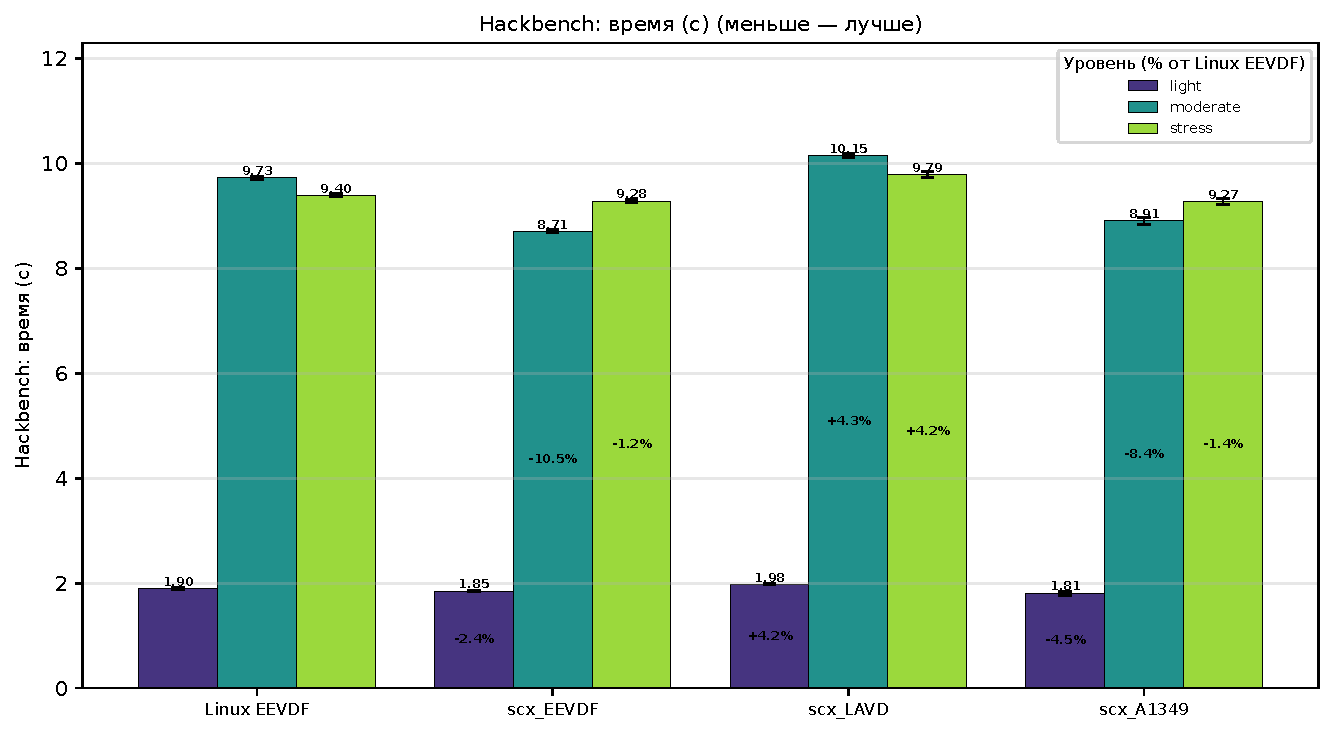
\includegraphics[width=0.9\textwidth]{res/bar_hackbench_time_sec.pdf}
                \caption{Время выполнения hackbench (секунды) для четырёх планировщиков по трём режимам нагрузки}
                \label{fig:bar_hackbench}
        \end{figure}

        \begin{figure}[H]
                \centering
                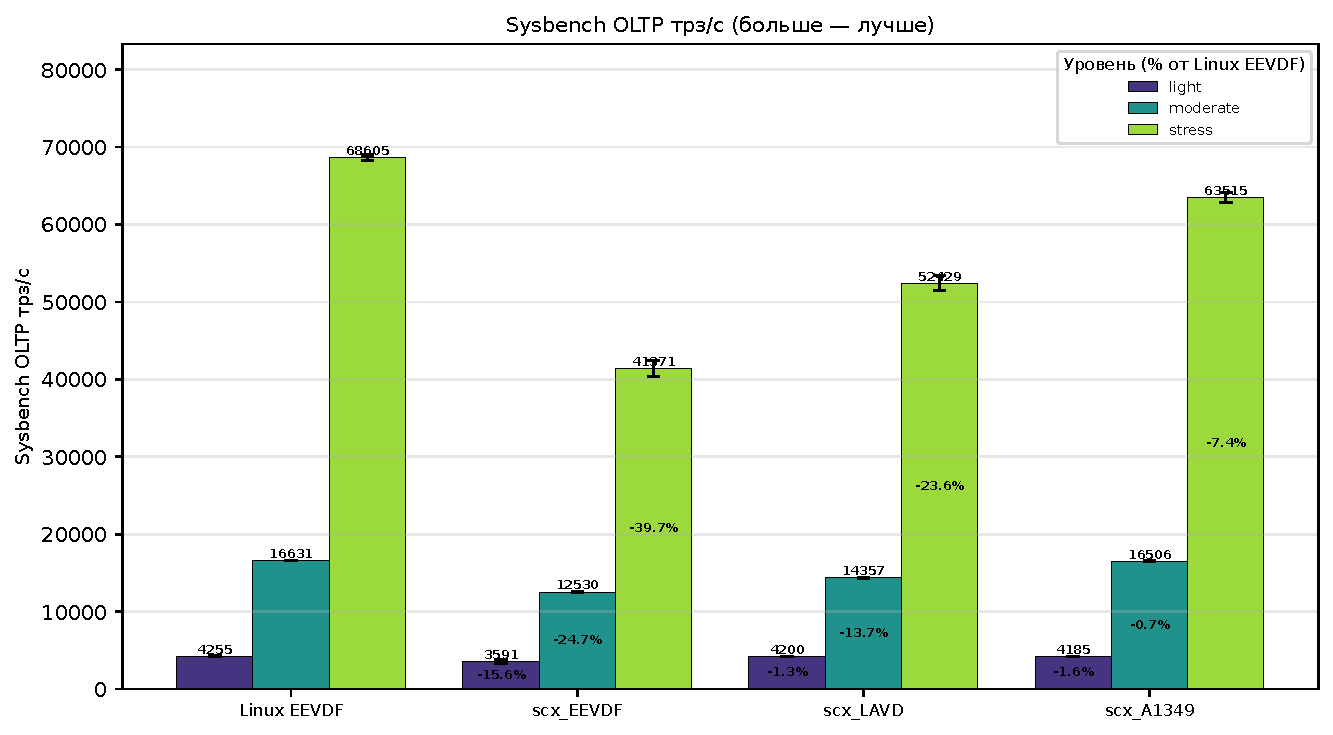
\includegraphics[width=0.9\textwidth]{res/bar_sysbench_tps.pdf}
                \caption{Пропускная способность sysbench (TPS) для четырёх планировщиков по трём режимам нагрузки}
                \label{fig:bar_sysbench_tps}
        \end{figure}

        \begin{figure}[H]
                \centering
                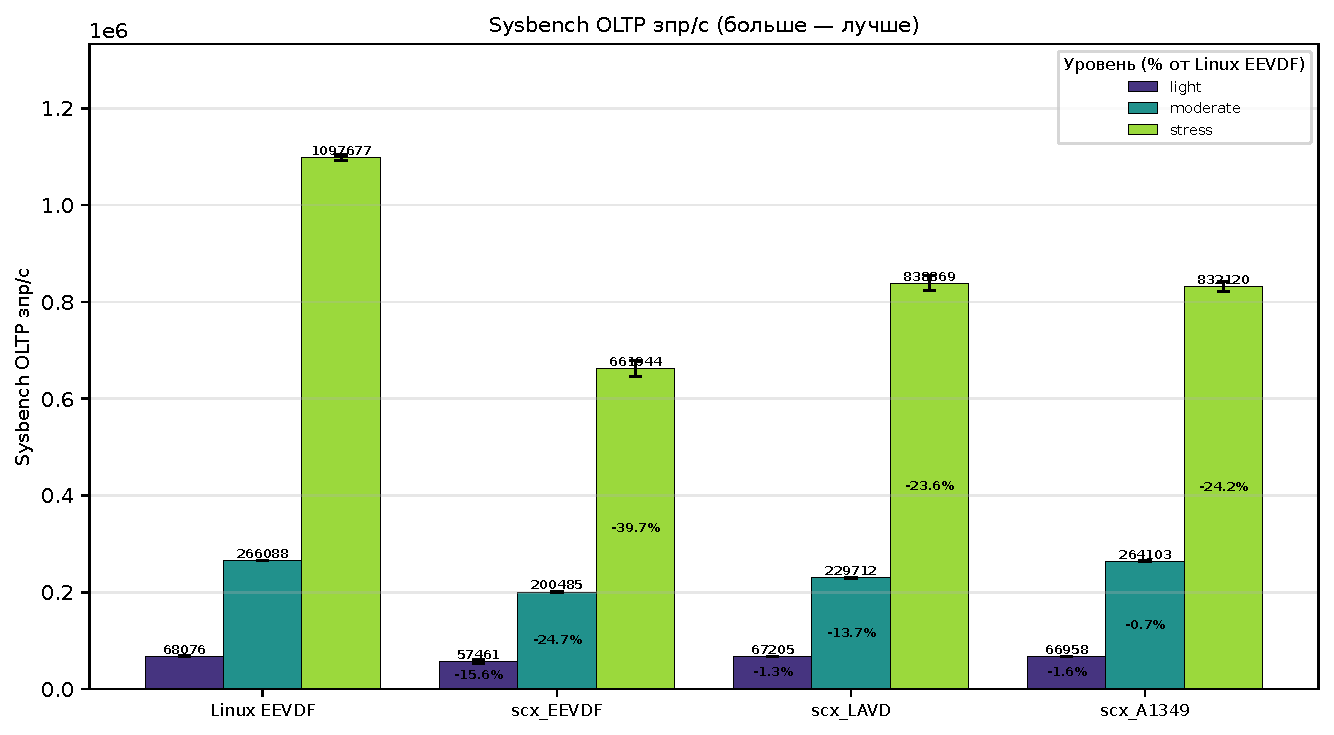
\includegraphics[width=0.9\textwidth]{res/bar_sysbench_qps.pdf}
                \caption{Пропускная способность sysbench (QPS) для четырёх планировщиков по трём режимам нагрузки}
                \label{fig:bar_sysbench_qps}
        \end{figure}

        \begin{figure}[H]
                \centering
                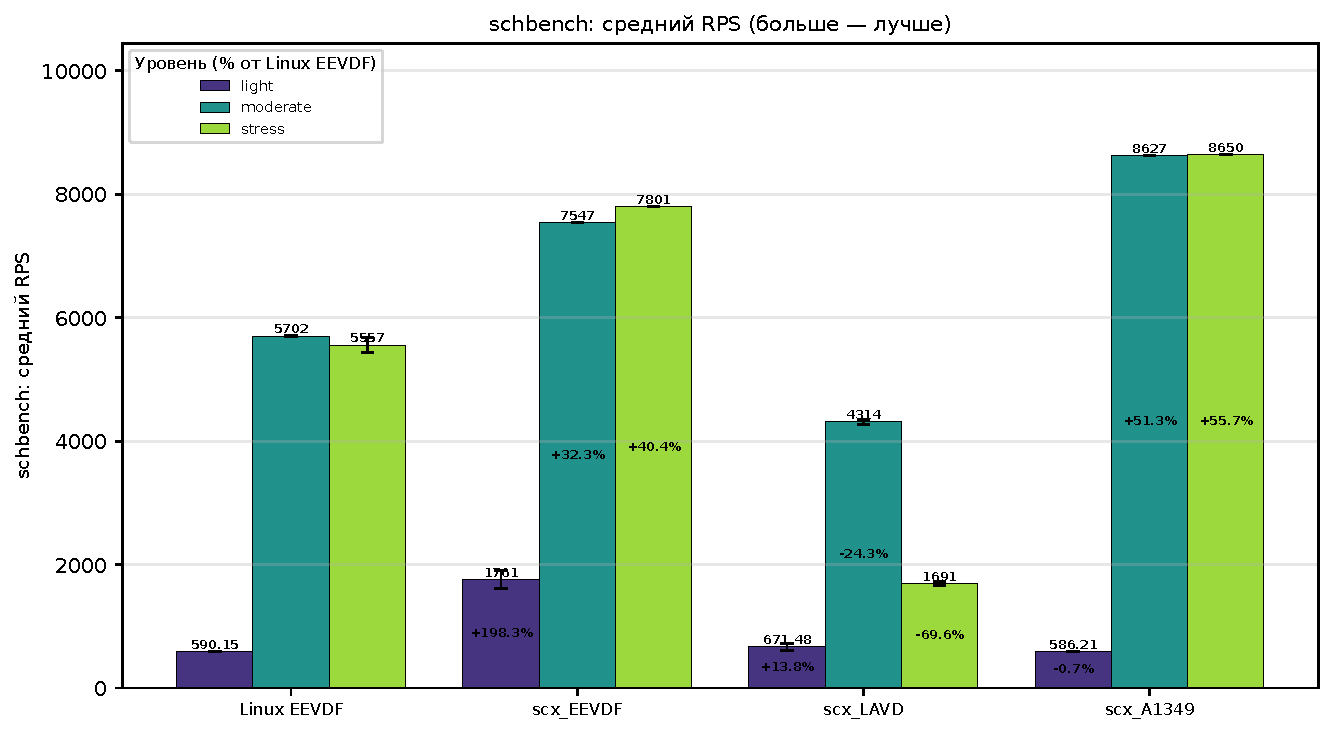
\includegraphics[width=0.9\textwidth]{res/bar_schbench_avg_rps.pdf}
                \caption{Средняя пропускная способность schbench (запросов в секунду) для четырёх планировщиков по трём режимам нагрузки}
                \label{fig:bar_schbench_avg_rps}
        \end{figure}

        \begin{figure}[H]
                \centering
                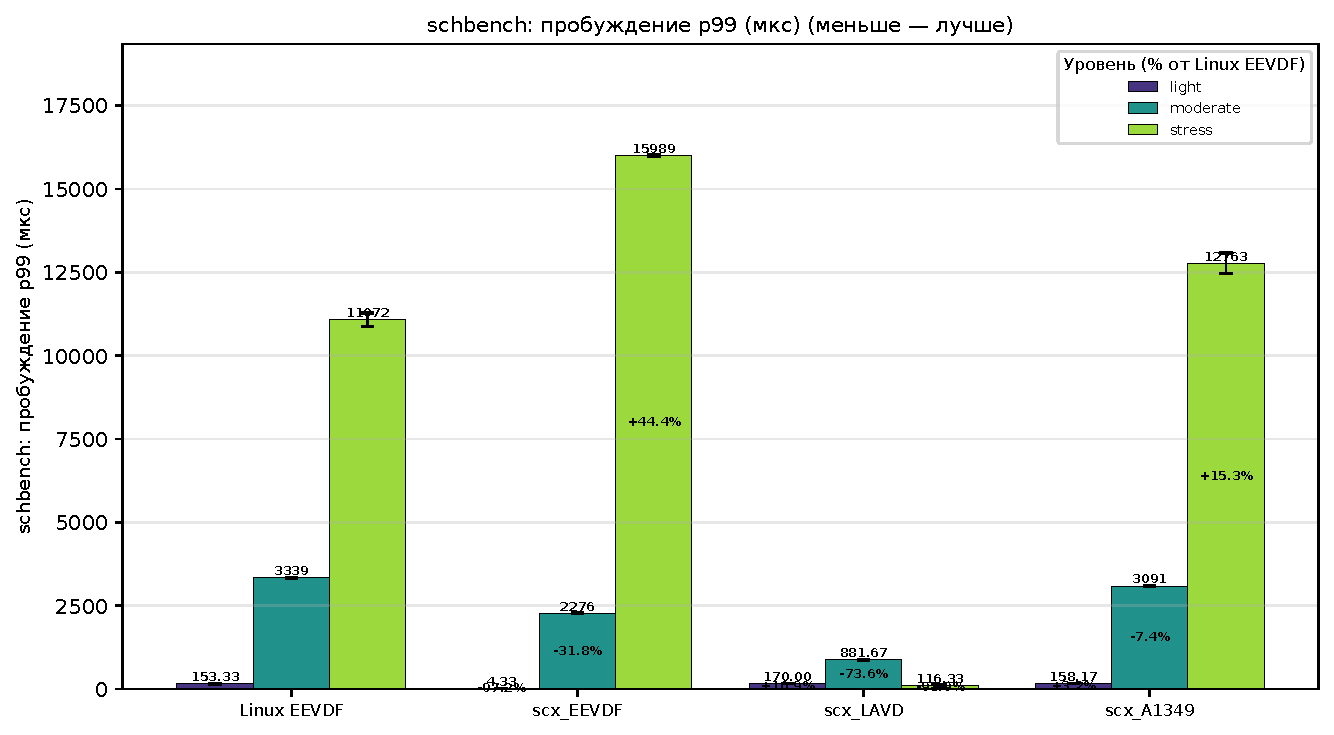
\includegraphics[width=0.9\textwidth]{res/bar_schbench_wakeup_p99_0_usec.pdf}
                \caption{Задержка пробуждения p99 schbench (мкс) для четырёх планировщиков по трём режимам нагрузки}
                \label{fig:bar_wakeup_p99}
        \end{figure}

        \begin{figure}[H]
                \centering
                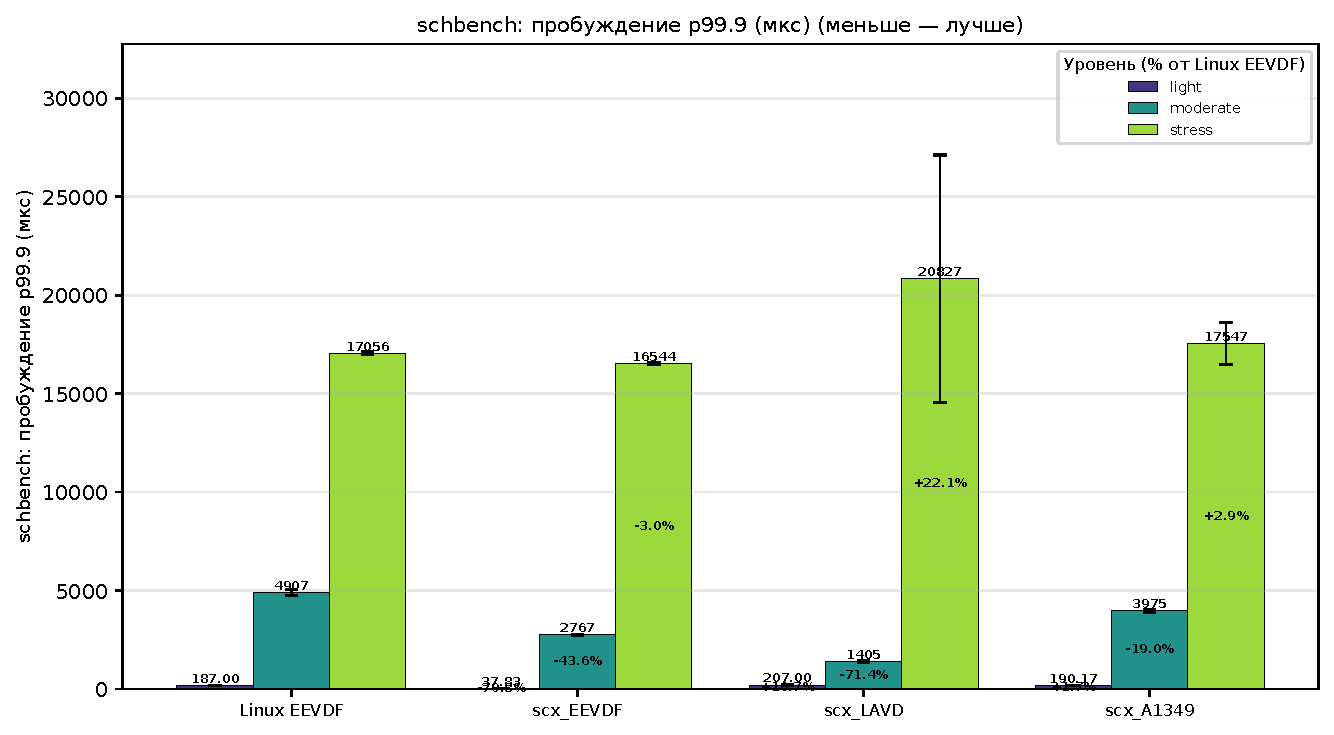
\includegraphics[width=0.9\textwidth]{res/bar_schbench_wakeup_p99_9_usec.pdf}
                \caption{Задержка пробуждения p99.9 schbench (мкс) для четырёх планировщиков по трём режимам нагрузки}
                \label{fig:bar_wakeup_p99_9}
        \end{figure}

        \begin{figure}[H]
                \centering
                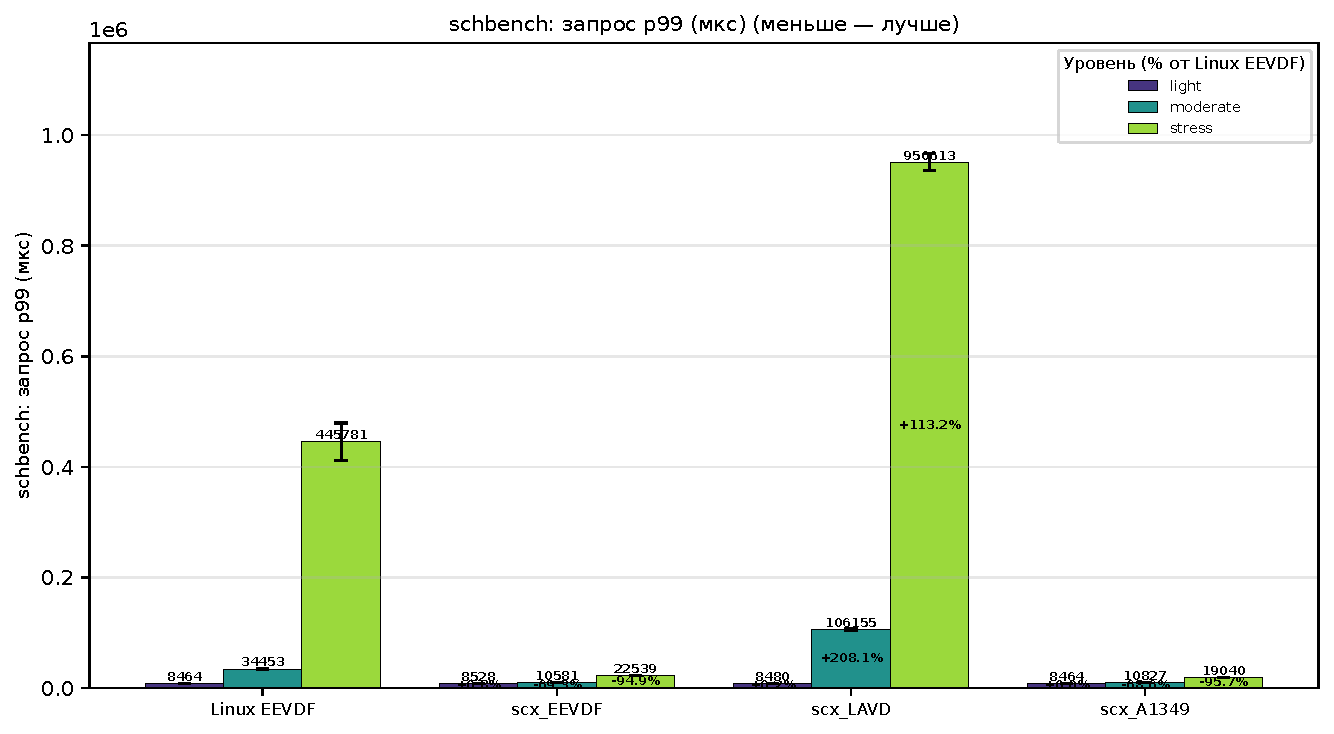
\includegraphics[width=0.9\textwidth]{res/bar_schbench_request_p99_0_usec.pdf}
                \caption{Задержка запроса p99 schbench (мкс) для четырёх планировщиков по трём режимам нагрузки}
                \label{fig:bar_request_p99}
        \end{figure}

        \begin{figure}[H]
                \centering
                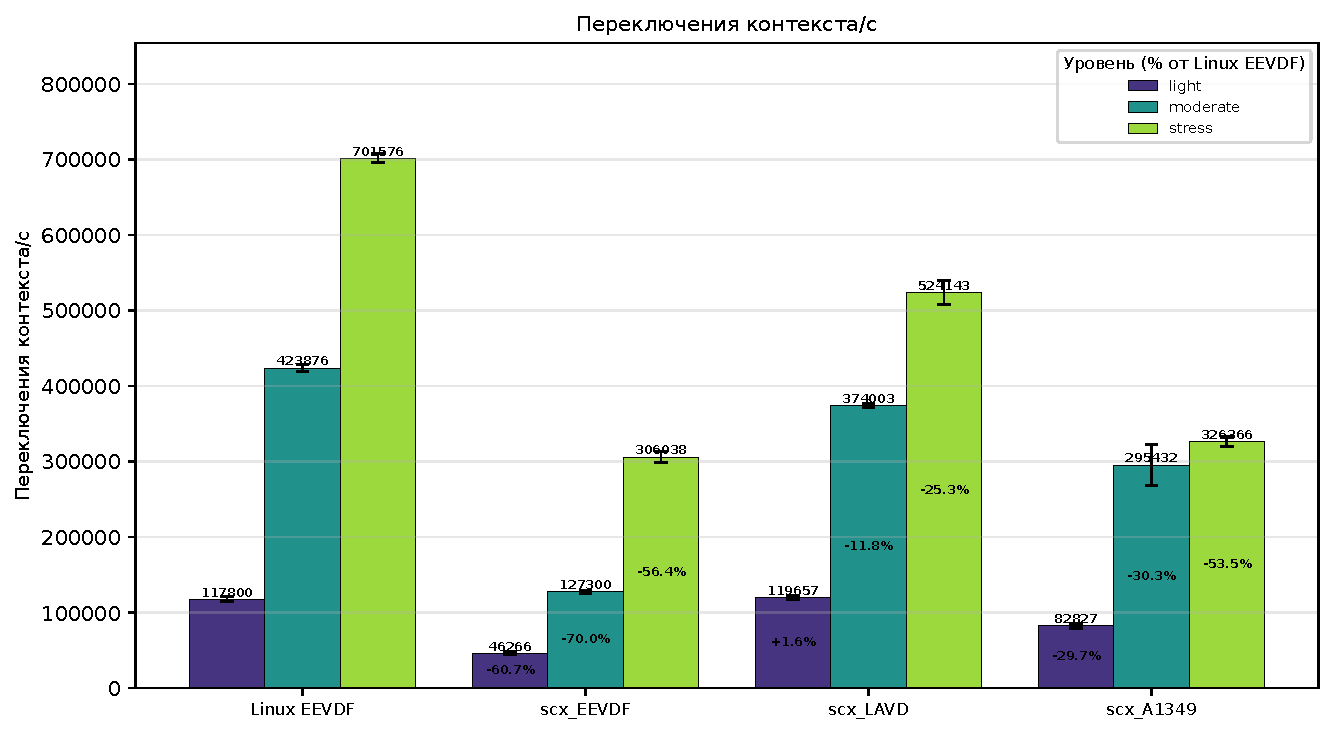
\includegraphics[width=0.9\textwidth]{res/bar_ctx_switches_per_sec.pdf}
                \caption{Темп переключений контекста (число в секунду) для четырёх планировщиков по трём режимам нагрузки}
                \label{fig:bar_ctx_switches}
        \end{figure}

        \begin{figure}[H]
                \centering
                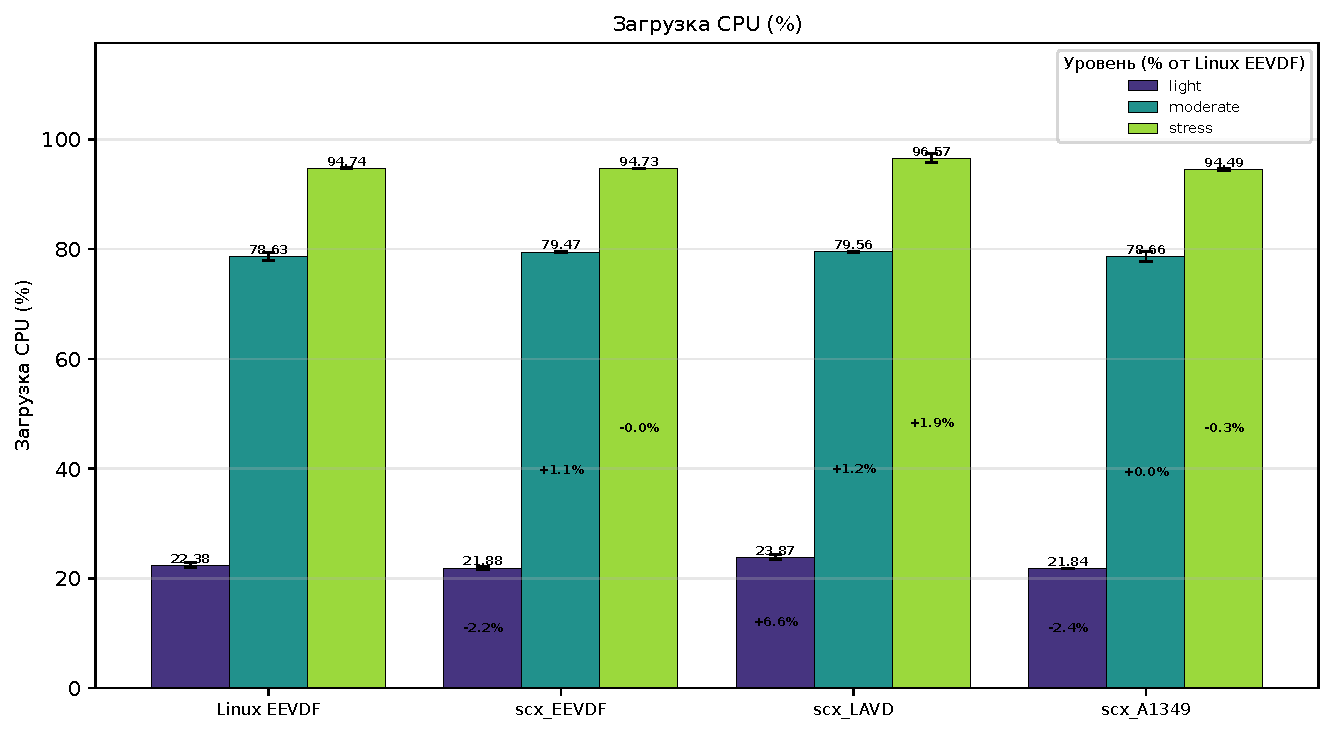
\includegraphics[width=0.9\textwidth]{res/bar_cpu_util_pct.pdf}
                \caption{Среднее использование CPU (\%) для четырёх планировщиков по трём режимам нагрузки}
                \label{fig:bar_cpu_util}
        \end{figure}

        \begin{figure}[H]
                \centering
                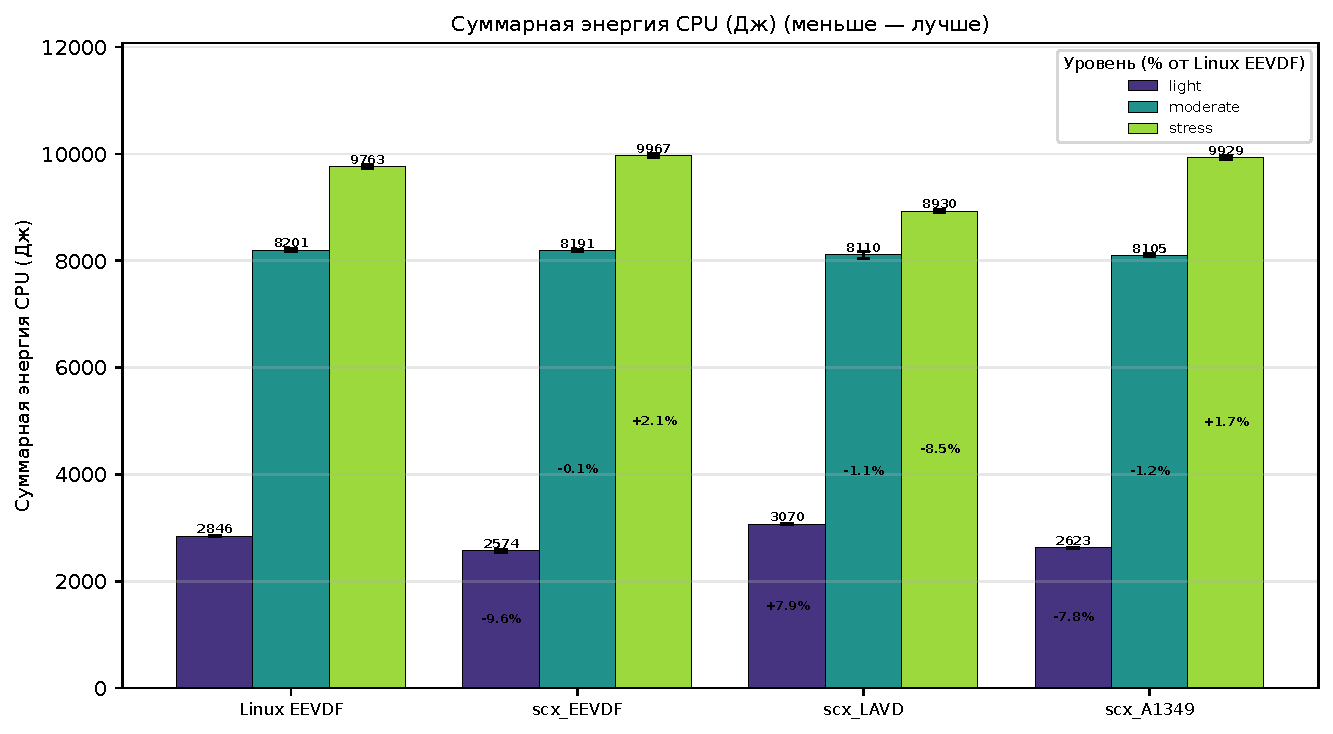
\includegraphics[width=0.9\textwidth]{res/bar_total_energy_joules.pdf}
                \caption{Суммарное энергопотребление (Дж) для четырёх планировщиков по трём режимам нагрузки}
                \label{fig:bar_energy}
        \end{figure}


\chapter*{Выводы}

        Проведённый эксперимент позволяет сформулировать
        основные закономерности поведения планировщика
        \texttt{scx\_A1349} на гетерогенной платформе в
        сравнении со штатным EEVDF, реализацией ядра
        алгоритма EEVDF поверх sched\_ext
        (\texttt{scx\_EEVDF}) и планировщиком LAVD.

        \textbf{Преимущества модели \texttt{scx\_A1349}.}
        На бенчмарке hackbench планировщик \texttt{scx\_A1349}
        опережает штатный EEVDF на всех трёх уровнях нагрузки:
        на $4{,}5$\,\% при лёгкой, на $8{,}5$\,\% при умеренной
        и на $1{,}4$\,\% при стрессовой. При лёгкой и
        стрессовой нагрузке \texttt{scx\_A1349} занимает
        первое место по среднему среди всех четырёх
        планировщиков, однако в обоих этих режимах его
        доверительный интервал пересекается с интервалом
        \texttt{scx\_EEVDF}, поэтому различие между ними
        статистически не значимо. Результат объясняется тем, что
        аукционный механизм направляет короткоживущие задачи
        hackbench преимущественно на P-ядра, где они
        завершаются быстрее.

        По пропускной способности schbench (средний RPS)
        планировщик \texttt{scx\_A1349} лидирует при умеренной
        ($8627$) и стрессовой ($8650$) нагрузке: на $51{,}3$\,\%
        выше штатного EEVDF при умеренной и на $55{,}7$\,\% при
        стрессовой нагрузке. При стрессовой нагрузке
        \texttt{scx\_A1349} показывает наименьшие значения p99
        и p99.9 задержки обслуживания запроса ($19{,}04$\,мс и
        $24{,}51$\,мс соответственно) среди всех планировщиков. Это может объясняться тем, что
        аукцион направляет задачи, чувствительные к задержке,
        на P-ядра, а бюджетные ограничения не дают отдельным
        задачам надолго блокировать остальные.

        Энергопотребление \texttt{scx\_A1349} относительно
        штатного EEVDF составляет $-7{,}8$\,\% при лёгкой
        нагрузке, $-1{,}2$\,\% при умеренной и $+1{,}7$\,\%
        при стрессовой. Источник этой зависимости от уровня
        нагрузки требует дополнительного анализа.

        \textbf{Ограничения модели \texttt{scx\_A1349}.}
        На бенчмарке sysbench при стрессовой нагрузке
        \texttt{scx\_A1349} отстаёт от штатного EEVDF на
        $7{,}4$\,\% ($63\,515$ TPS против $68\,605$ TPS).
        Аналогичное, но меньшее отставание ($1{,}6$\,\% при
        лёгкой и $0{,}8$\,\% при умеренной) сохраняется на
        других уровнях нагрузки.
        При этом \texttt{scx\_A1349} существенно превосходит
        вторую sched\_ext-реализацию (\texttt{scx\_EEVDF}) во
        всех режимах. Часть отставания от штатного EEVDF
        обусловлена накладными расходами sched\_ext при
        высоком темпе переключений контекста.

        По хвостовой задержке пробуждения при лёгкой нагрузке
        \texttt{scx\_A1349} уступает \texttt{scx\_EEVDF}
        более чем на порядок (p99 $158$\,мкс против $4$\,мкс).
        Поскольку оба планировщика построены на sched\_ext,
        различие, по-видимому, обусловлено дополнительной
        логикой выбора ядра в \texttt{scx\_A1349} (поиск
        свободного P-ядра при пробуждении), которая при
        отсутствии конкуренции увеличивает время пробуждения,
        не давая выигрыша от назначения на более производительное
        ядро.

        \textbf{Влияние свойств модели на результаты.}
        Учёт типа ядра при назначении задач, заложенный в
        модель A1349, наиболее заметен в режимах умеренной и
        стрессовой нагрузки: \texttt{scx\_A1349} лидирует по
        средней пропускной способности schbench ($8627$ и
        $8650$ запросов в секунду соответственно) и сокращает
        время выполнения hackbench относительно штатного EEVDF
        на всех трёх уровнях нагрузки. При стрессовой нагрузке
        хвостовая задержка обслуживания запроса p99.9 составляет
        $24{,}51$\,мс у \texttt{scx\_A1349} против
        $\approx$\,$1{,}69$\,с у штатного EEVDF и
        $\approx$\,$1{,}81$\,с у LAVD. Близкое значение
        \texttt{scx\_EEVDF} ($27{,}21$\,мс) показывает, что
        этот эффект во многом связан с самим sched\_ext, а не
        исключительно с аукционным механизмом A1349.

        \textbf{Ограничения эксперимента.}
        Все планировщики тестировались с $n = 6$ запусками на
        фиксированной длительности. Эксперимент проведён на
        единственной аппаратной платформе (Intel Arrow Lake-S),
        и переносимость результатов на архитектуры ARM
        big.LITTLE и RISC-V требует дополнительной проверки.
        Кроме того, использованные бенчмарки не покрывают
        все возможные сценарии использования оборудования.
        Вклад отдельных механизмов \texttt{scx\_A1349}
        (аукционный платёж, предпочтение P-ядер при
        пробуждении, корзина токенов бюджета, привязанные
        к ядрам очереди, ускоренный путь диспетчеризации)
        не разделён экспериментально и требует отдельной
        серии замеров с поочерёдным отключением механизмов.


\chapter*{Заключение}

        В работе предложен и реализован планировщик для
        гетерогенных архитектур, проведена его экспериментальная
        оценка на реальной аппаратной платформе. Выполнен обзор
        подходов к реализации планировщиков в операционных
        системах и обоснован выбор фреймворка sched\_ext.

        Построена математическая модель A1349 на основе
        динамического VCG-механизма, трактующая выбор ядра для
        задачи как исход аукциона. Эффективная ценность задачи
        учитывает стоимость кванта целевого ядра, отражая
        разницу производительности P/E ядер. Аукцион назначает задачу на тот тип ядра,
        где её эффективная ценность максимальна, VCG-платёж
        задаёт цену вытеснения конкурента, а бюджетные
        ограничения предотвращают монополизацию
        производительных ядер.

        Модель и алгоритм EEVDF реализованы средствами
        sched\_ext, что позволило сравнить A1349 со штатным
        EEVDF, реализацией EEVDF в sched\_ext
        (\texttt{scx\_EEVDF}) и LAVD. Подготовлена
        воспроизводимая методика измерений на основе
        бенчмарков hackbench, sysbench и schbench при трёх
        уровнях нагрузки, и
        проведён эксперимент на платформе Intel Arrow Lake-S
        с P/E ядрами.

        На hackbench \texttt{scx\_A1349} опережает штатный
        EEVDF на всех уровнях нагрузки: на $4{,}5$\,\% при
        лёгкой, на $8{,}5$\,\% при умеренной и на $1{,}4$\,\%
        при стрессовой. На schbench при умеренной и стрессовой
        нагрузке он лидирует по средней пропускной способности
        ($+51{,}3$\,\% и $+55{,}7$\,\% относительно штатного
        EEVDF). По хвостовой задержке при стрессовой нагрузке
        (p99.9) \texttt{scx\_A1349}
        опережает штатный EEVDF и LAVD на два порядка
        ($24{,}51$\,мс против $\approx$\,$1{,}69$\,с и
        $\approx$\,$1{,}81$\,с). На sysbench все
        sched\_ext-планировщики отстают от штатного EEVDF,
        что указывает на накладные расходы фреймворка.

        Эксперимент показал, что учёт гетерогенности на уровне
        математической модели даёт измеримый выигрыш на
        нагрузках, где размещение задач по типам ядер влияет на
        результат.

        Перспективными направлениями являются переносимость
        модели A1349 на ARM big.LITTLE и RISC-V и обобщение
        на конфигурации с более чем двумя типами ядер
        (Intel P/E/LPE).


\renewcommand{\bibname}{Список литературы}
\begin{thebibliography}{9}
        \vspace*{0.3cm}

        \bibitem{lions}
        Lions~J. A Commentary on the Sixth Edition UNIX Operating
        System. --- Sydney: The University of New South Wales, 1977.

        \bibitem{kravetz_elss}
        Kravetz~M., Franke~H., Nagar~S., Ravindran~R. Enhancing Linux
        Scheduler Scalability // Proceedings of the Ottawa Linux
        Symposium. --- 2001.

        \bibitem{love}
        Love~R. Linux Kernel Development. --- 2nd ed. --- Indianapolis:
        Novell Press, 2005. --- 401~p.

        \bibitem{wong}
        Wong~C.~S., Tan~I.~K.~T., Kumari~R.~D., Lam~J.~W., Fun~W.
        Fairness and Interactive Performance of O(1) and CFS Linux
        Kernel Schedulers // International Symposium on Information
        Technology (ITSim 2008). --- Kuala Lumpur: IEEE, 2008. ---
        P.~1--6.

        \bibitem{stoica}
        Stoica~I., Abdel-Wahab~H. Earliest Eligible Virtual Deadline
        First: A Flexible and Accurate Mechanism for Proportional Share
        Resource Allocation: Technical Report TR-95-22. --- Norfolk:
        Old Dominion University, 1995.

        \bibitem{biglittle}
        Greenhalgh~P. Big.LITTLE Processing with ARM Cortex-A15 \&
        Cortex-A7: ARM White Paper. --- Cambridge: ARM Ltd., 2011.

        \bibitem{intelhybrid}
        Rotem~E. et al. Alder Lake Architecture // 2021 IEEE Hot Chips
        33 Symposium (HCS). --- Palo Alto, CA, USA, 2021. ---
        P.~1--23. --- DOI:~10.1109/HCS52781.2021.9567097.

        \bibitem{marsellus}
        Conti~F., Paulin~G., Garofalo~A., Rossi~D., Di~Mauro~A.,
        Rutishauser~G., Ottavi~G., Eggimann~M., Okuhara~H., Benini~L.
        Marsellus: A Heterogeneous RISC-V AI-IoT End-Node SoC with
        2-to-8b DNN Acceleration and 30\%-Boost Adaptive Body
        Biasing // IEEE Journal of Solid-State Circuits. --- 2024. ---
        Vol.~59, No.~1. --- P.~128--142.

        \bibitem{eas}
        Energy Aware Scheduling [Электронный ресурс] // Linux Kernel
        Documentation. --- URL:
        \url{https://www.kernel.org/doc/html/latest/scheduler/sched-energy.html}
        (дата обращения: 14.11.2025).

        \bibitem{schedext}
        Corbet~J. The BPF extensible scheduler class [Электронный
        ресурс] // LWN.net. --- 30.11.2022. --- URL:
        \url{https://lwn.net/Articles/916291/}
        (дата обращения: 20.11.2025).

        \bibitem{lwn_schedext_lpc}
        Corbet~J. Sched\_ext at LPC 2024 [Электронный ресурс] //
        LWN.net. --- 2024. --- URL:
        \url{https://lwn.net/Articles/991205/}
        (дата обращения: 11.09.2025).

        \bibitem{ghost}
        Humphries~J.~T., Natu~N., Chaugule~A., Weisse~O., Rhoden~B.,
        Don~J., Rizzo~L., Rombakh~O., Turner~P., Kozyrakis~C. ghOSt:
        Fast \& Flexible User-Space Delegation of Linux Scheduling //
        Proceedings of the 28th ACM Symposium on Operating Systems
        Principles (SOSP 2021). --- New York: ACM, 2021. ---
        P.~588--604.

        \bibitem{srand}
        Tang~Q., Gao~X., Li~G., Lin~J. Optimizing Linux Scheduling Based
        on Global Runqueue with SCX // IEEE International Conference on
        Systems, Man, and Cybernetics (SMC 2024). --- IEEE, 2024.

        \bibitem{lace}
        Xu~J., Wolff~D., Han~X.~Y., Li~J., Roychoudhury~A. Concurrency
        Testing in the Linux Kernel via eBPF: preprint. --- arXiv,
        2025. --- arXiv:2504.21394.

        \bibitem{aegis}
        Mao~J., Ujcich~B.~E., Ma~S. Rethinking Provenance Completeness
        with a Learning-Based Linux Scheduler: preprint. --- arXiv,
        2025. --- arXiv:2510.08479.

        \bibitem{mos}
        Wang~X., Jia~S., Huang~Z., Cao~J., Song~M. Mixture-of-Schedulers:
        An Adaptive Scheduling Agent as a Learned Router for Expert
        Policies: preprint. --- arXiv, 2025. --- arXiv:2511.11628.

        \bibitem{lavd}
        Galin~M., Hedblom~A. Linux Kernel Scheduler Evaluation for
        Performance-Critical Telecom Workloads: Master's Thesis. ---
        Linköping: Linköping University, 2025. --- 74~p.

        \bibitem{pie}
        Van~Craeynest~K., Jaleel~A., Eeckhout~L., Narvaez~P.,
        Emer~J.~S. Scheduling Heterogeneous Multi-Cores through
        Performance Impact Estimation (PIE) // Proceedings of the 39th
        Annual International Symposium on Computer Architecture (ISCA
        2012). --- New York: ACM, 2012. --- P.~213--224.

        \bibitem{sano}
        Sano~R. A Dynamic Mechanism Design for Scheduling with Different
        Use Lengths: KIER Discussion Paper No.~924. --- Kyoto: Institute
        of Economic Research, Kyoto University, 2015.

        \bibitem{dln}
        Dobzinski~S., Lavi~R., Nisan~N. Multi-unit Auctions with Budget
        Limits // Games and Economic Behavior. --- 2012. ---
        Vol.~74, No.~2. --- P.~486--503.

\end{thebibliography}

\end{document}
